\documentclass[10pt]{article} % Font size - 10pt, 11pt or 12pt

\usepackage[hmargin=1.25cm, vmargin=1.5cm]{geometry} % Document margins
\usepackage[usenames,dvipsnames]{xcolor} % Allows the definition of hex colors

\usepackage{listings}
\lstset{escapechar=\&}

% Fonts and tweaks for XeLaTeX
\usepackage{fontspec,xltxtra,xunicode}
\defaultfontfeatures{Mapping=tex-text}
%\setmonofont[Scale=MatchLowercase]{Andale Mono}

% Colors for links, text and headings
\usepackage{hyperref}
\definecolor{linkcolor}{HTML}{506266} % Blue-gray color for links
\definecolor{shade}{HTML}{F5DD9D} % Peach color for the contact information box
\definecolor{text1}{HTML}{2b2b2b} % Main document font color, off-black
\definecolor{headings}{HTML}{701112} % Dark red color for headings
% Other color palettes: shade=B9D7D9 and linkcolor=A40000; shade=D4D7FE and linkcolor=FF0080

\hypersetup{colorlinks,breaklinks, urlcolor=linkcolor, linkcolor=linkcolor} % Set up links and colors

\usepackage{titlesec}
\setcounter{secnumdepth}{4}

\titleformat{\paragraph}
{\normalfont\normalsize\bfseries}{\theparagraph}{1em}{}
\titlespacing*{\paragraph}
{0pt}{3.25ex plus 1ex minus .2ex}{1.5ex plus .2ex}

\usepackage{fancyhdr}
\usepackage{amssymb}
\usepackage{amsmath}
\pagestyle{fancy}
\fancyhf{}

\renewcommand{\headrulewidth}{0pt} % Get rid of the default rule in the header

\bibliographystyle{plain}

\begin{document}

\tableofcontents
\newpage

\section{Chapter: Introduction}
\subsection{What is dynein?}
\subsubsection{Basics}

Dynein is a cellular structure which converts chemical energy to mechanical energy. It does so by reacting with adenosine triphosphate (ATP) to take steps along long cellular tracks known as microtubules (MTs). Dynein's mechanical energy is used to transport molecules around the cell, pull chromosomes during division, move cellular propellers known as cilia and various other functions \cite{cianfroccoreview}.\\

Dynein is a protein with many smaller domains. A depiction of the protein and its labeled subdomains is shown in Figure (\ref{dynein-artist-rendition}). Each motor is a homodimer made up of two identical monomer proteins. Each monomer has a binding domain which binds to the microtubule, a motor domain which binds ATP, a tail domain which connects to the other monomer, a stalk which connects the binding and motor domains, and a linker which connects the motor and tail domains. The tail domain is also responsible for binding to cargo.\\

\begin{figure}[h]
  \centering
  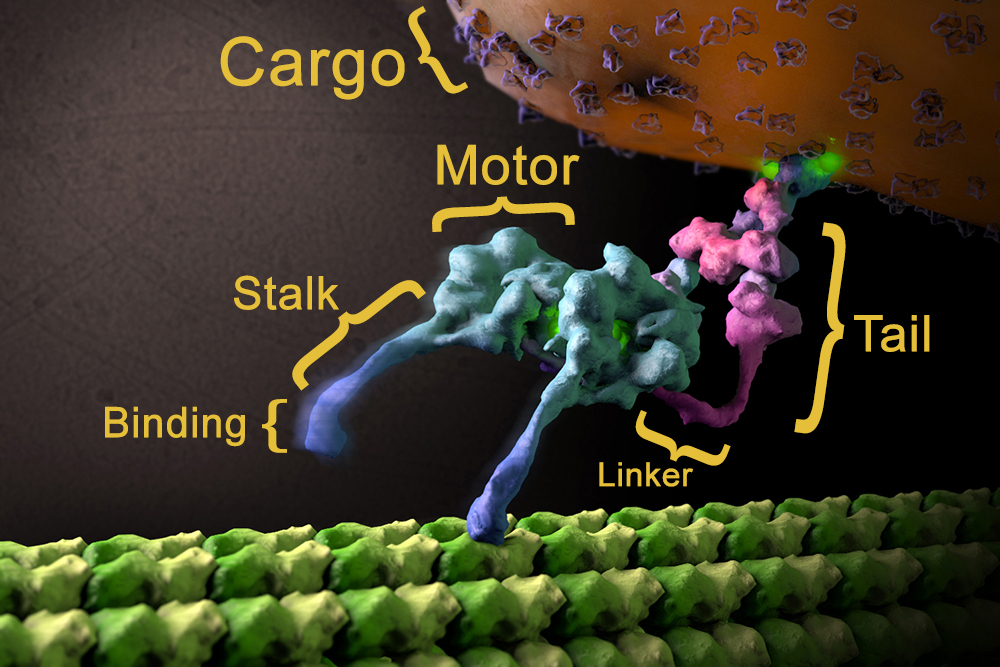
\includegraphics[width=.65\textwidth,keepaspectratio]{../figures/dynein-artist-rendition.jpg}
  \caption{Artist rendition of the dynein motor bound to a microtubule. One monomer is bound to the MT, and one is raised up. Modified. Source: Lander Lab, The Scripps Research Institute.}
  \label{dynein-artist-rendition}
\end{figure}

Dynein is believed to move by using the energy of ATP to cycle through a ring of states, each with different spatial relations to the microtubule. By cycling forward through this ring, the molecule can end up in the same state it began, but moved forward a small amount. This ring of states is known as the mechanochemical cycle \cite{cianfroccoreview}. The goal of this project is to create a mathematical model of the mechanochemical cycle and verify that it can reproduce experimental dynein stepping data. There are several types of dynein which all behave differently. This project will focus on cytoplasmic dynein-1, hereby referred to as dynein.\\

\subsubsection{Glossary}
\textbf{ATP} Adenosine triphosphate is a small organic molecule which very spontaneously breaks apart into ADP and a phosphate. This reaction is used to power many energy-requiring mechanisms within the cell. This reaction has a $\Delta G^\circ \approx -36 kJ/mol$ at physiological conditions \ref{ATPenergy}.\\\\
\textbf{Protein} Dynein is a protein, or long chain of amino acids linked together and folded into a particular shape.\\

\subsubsection{Why do cells need motor transport?}
Cells are organized, heretogenous structures which respond quickly to their environments. This means that cells require a mechanism for rapidly moving components to precise locations within the cell. This can be a challenge, since cells are fairly large compared to the proteins which compose them. A human fibroblast cell has a volume of roughly 2000 $\mu m^3$\cite{fibroblastvolume}, corresponding to roughly $8 \mu m$ in diameter. In comparison, human hemoglobin has a diameter of roughly $5 nm$ (PDB id 5ME2) \textbf{((is this the best way to cite this?))}, a $10^3$ factor difference in size.\\

Diffusion, or random motion of molecules due to collisions with solvent (i.e. Brownian motion), is one possible process cells could use to transport biomolecules. Diffusion has two problems: it is slow and nondirected. The expected distance covered for one-dimensional Brownian motion after time t was found by Einstein to be \textbf{cite here}:

\begin{equation}
  \label{diffusion-equation}
  <x> = \sqrt{2Dt}
\end{equation}

where D is the diffusion constant describing the diffusability of the biomolecule. For a medium-sized (140kD, 1D = weight of H atom) protein with a diffusion constant $D = .2 \mu m^2/s$ %% \cite{diffusionconstants}
, it would take about a month to travel across a millimeter-sized cell. In contrast, it would take dynein, which travels at roughly 100nm/s \cite{weihongpaper}, a much more reasonable three hours to do the same.

\begin{figure}[h]
  \centering
  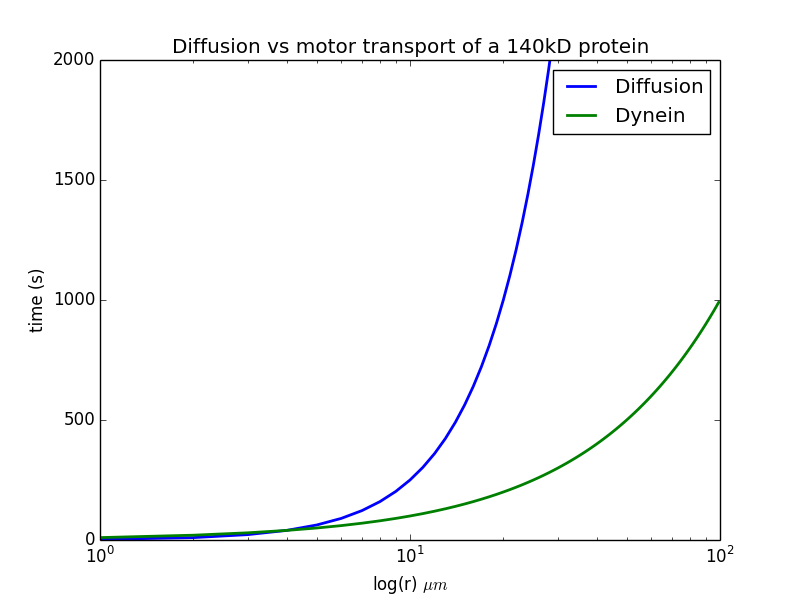
\includegraphics[width=.65\textwidth,keepaspectratio]{../figures/diffusion_vs_dynein.png}
  \caption{Plot comparing the diffusion rate of a 140kD protein with a diffusion consant $D = .2 \mu m^2/s$ with a dynein motor travelling at 100nm/s.}
  \label{diffusion_vs_dynein}
\end{figure}

\textit{Maybe use the more reasonable 2$\mu m / s$ number for dynein velocity, in-vitro speed may not be applicable since [ATP]-limited}

Another advantage of motor transport is that microtubules can be highly specific in their location in the cell. During cell division chromosomes line up at the center of each cell in a plane. Such a geometrically precise shape requires some sort of directed motion which a random process could never provide.\\

\textit{maybe decorate the above plot with pictures of cells of each size, or how long certain cellular events take? That could be cool and make it actually an interesting plot}
\textit{this argument would be much better if you could find examples of things which need to be done quickly in the cell, like responding to foreign particles or signalling
  molecules or cell division or neural events}

\subsubsection{What role does it play in the cell?}
Some of dynein's primary roles in the cell are to transport cellular cargos such as organelles, vesicles, mRNA, cytoskeletal filaments and certain proteins. Dynein also plays a role in positioning and breaking down the nucleus, cell death, spindle formation and the placement of other important cellular structures \cite{valetoolbox}.

Microtubules are long polymers of alternating $\alpha-$ and $\beta-$ tubulin subunits. MTs are polar, meaning they have a distinct directionality based on the orientation of thetubulin proteins which comprise them. One pole, the minus end, is where they initiate formation, typically at a MTOC (microtubule organizing center) around the center of the cell. The other pole, the plus end, is where they grow and shrink from. Kinesin and myosin, two other families of motor protein, typically walk towards the plus end of the MT. Dynein is unique in that it walks towards the minus end, making it a minus end-directed motor. This lends it to a particularly important function inside neurons known as retrograde transport.\\

Neurons have cell bodies at their centers and axons which grow outwards. Axons are long, narrow structures extending up to a meter in length in humans. Cell bodies contain nuclei and important organelles for synthesizing proteins, but growth of axon tips is vital for neuron function. This means bidirectional motor transport between axon tips and cell bodies is very important in neurons, since diffusion would not be quick enough. Retrograde transport is transport from the axon tip to the cell body. Cargo includes vesicles full of proteins ready to be broken down in the cell body and microtubule fragments to be returned from the axon tip \cite{neuroanatomy}. Because microtubule minus ends are found in the cell body, dynein's minus end-directed nature makes it the only protein capable of retrograde transport. An interesting question is, if proteins like dynein are synthesized in the cell body but needed at the axon tip to perform retrograde transport, how do dynein get to the tip? The answer is shown in \ref{retrograde-transport}: kinesin, a plus end-directed motor, takes dynein to the tip from the cell body.\\

\begin{figure}[h]
  \centering
  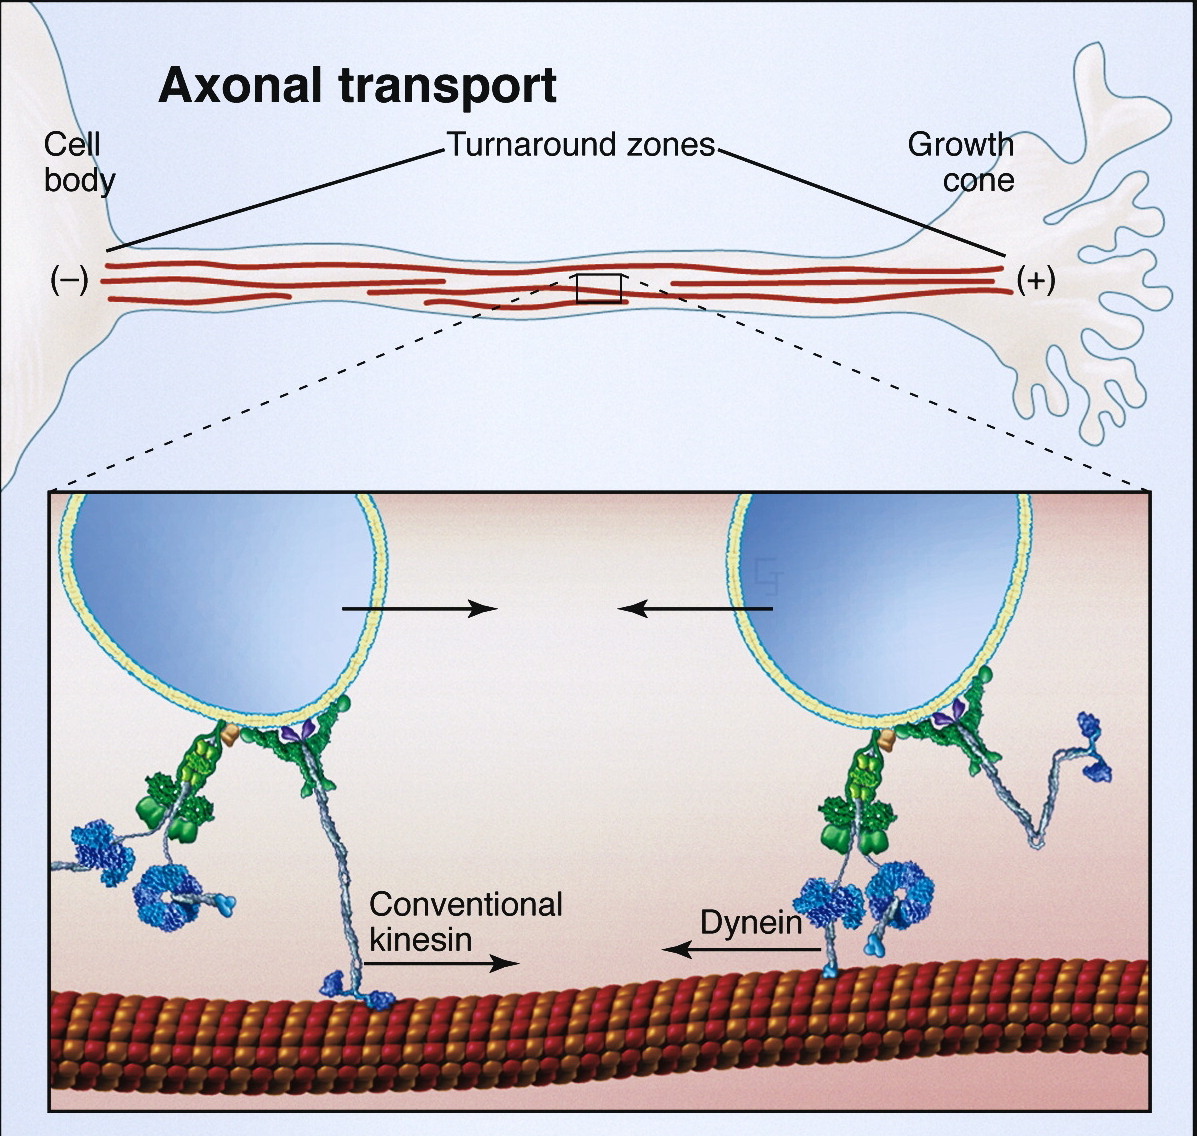
\includegraphics[width=.65\textwidth,keepaspectratio]{../figures/retrograde_transport.jpg}
  \caption{Mechanism of dynein localization to axon tips, or growth cones, in retrograde transport mediated by kinesin anterograde transport. Modified from \cite{valetoolbox}.}
  \label{retrograde-transport}
\end{figure}

\subsubsection{Dynein structure}

\begin{figure}[h]
  \centering
  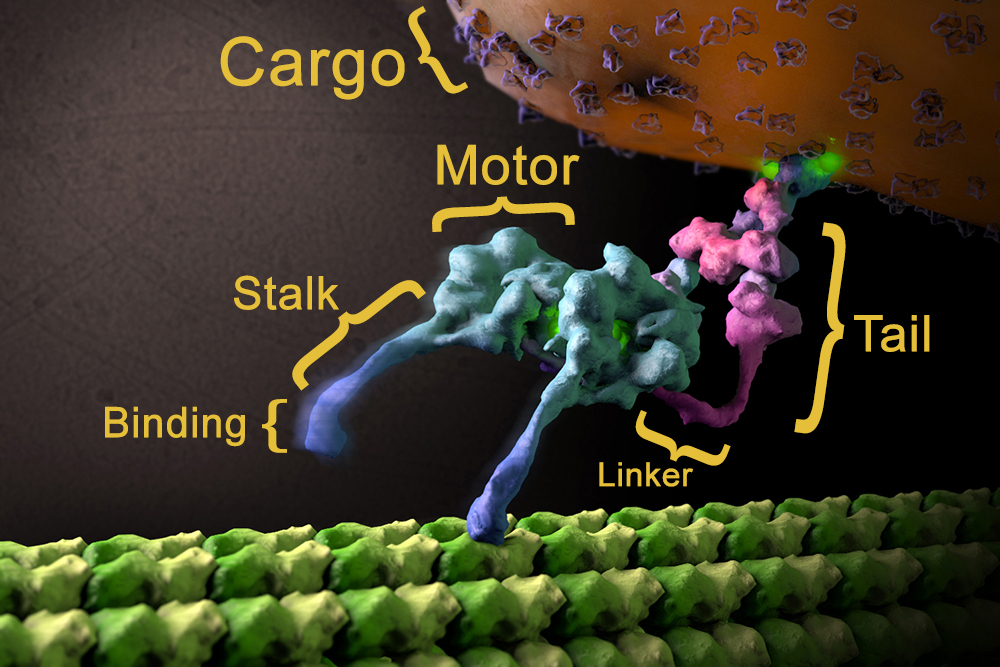
\includegraphics[width=.65\textwidth,keepaspectratio]{../figures/dynein-artist-rendition.jpg}
  \caption{Artist rendition of the dynein motor bound to a microtubule. One monomer is bound to the MT, and one is raised up. Modified. Source: Lander Lab, The Scripps Research Institute.}
  \label{dynein-artist-rendition-2}
\end{figure}

\textit{eventually find a different figure}

As shown in \ref{dynein-artist-rendition-2}, a dynein motor is a fusion of to identical subunits, or monomers, each with binding, stalk, motor and tail subdomains. Each of these subunits has a unique purpose for the motor.

\textbf{Binding domain}
Microtubule binding domains (MTBDs) allow dynein to bind to the microtubule. 

\begin{figure}[h]
  \centering
  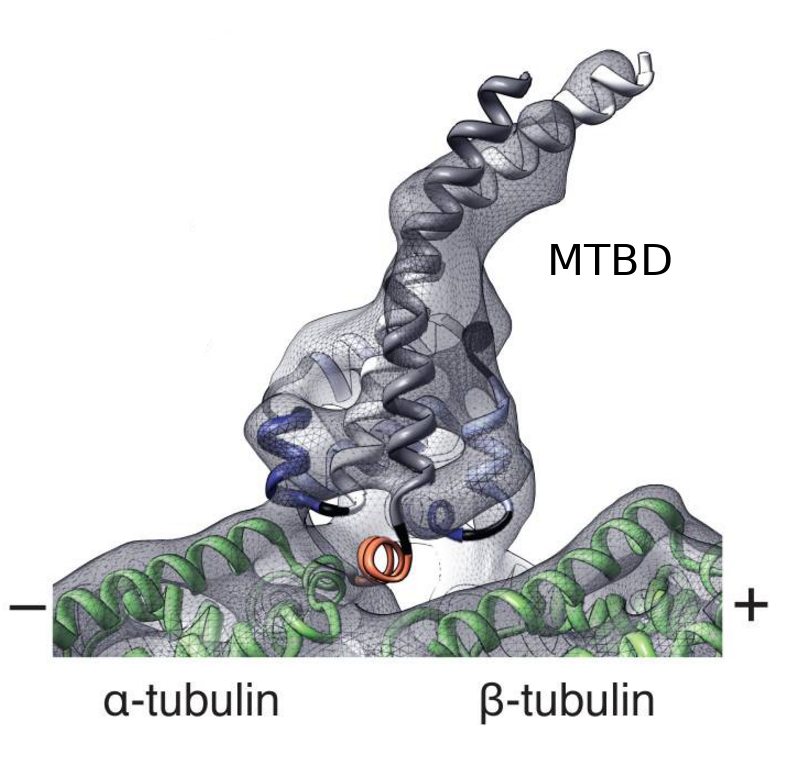
\includegraphics[width=.65\textwidth,keepaspectratio]{../figures/mtbd-complex.png}
  \caption{Crystal structure of the MTBD-MT complex. Modified from Redwine \textit{et. al} \cite{redwineMTBDcomplex}.}
  \label{dynein-artist-rendition-2}
\end{figure}

\subsubsection{How does it behave?}
Talk about its stepping behavior using Weihong's figures (as well as the new paper David found?)\\

Also possibly talk about the other things Dynein has been found to do, such as hydrolyse ATP and
move its subdomains around. This may be better in a different section than the introduction though,
since its a lot of biochemistry for the second section in an intro? maybe not, it has to go somewhere.

\subsubsection{Why is dynein special and interesting?}
Compare the processive motion of dynein to kinesin in \textbf{a.)} directionality, \textbf{b.)}
stepping pattern and \textbf{c.)} size (like how it can step over roadblocks kinesin cannot).\\

Talk about why a random stepping motor is interesting compared to a orderly-stepping motor: what
is different about dynein's structure that makes it step differently? Compare the crystal structures
and ask lots of questions. Build interest in the motors here.\\

%% \begin{figure}[h]
%%   \centering
%%   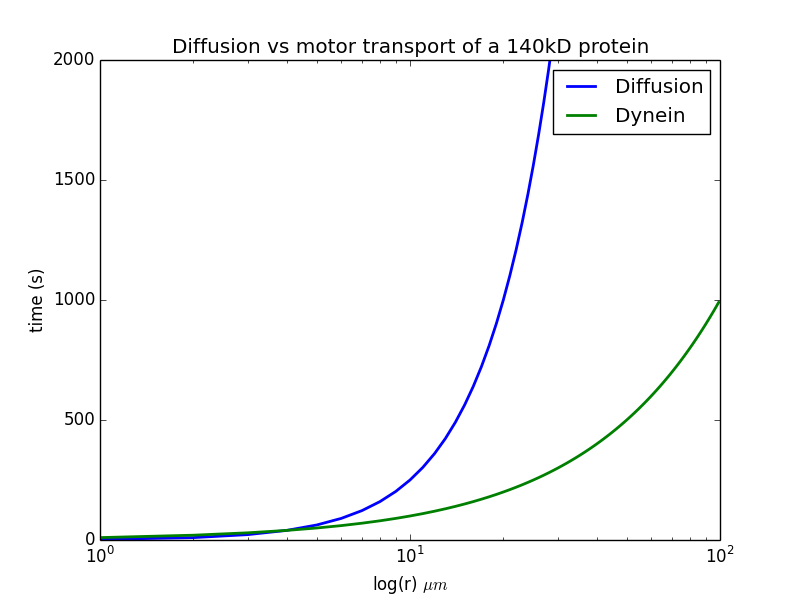
\includegraphics[width=.65\textwidth,keepaspectratio]{../figures/diffusion_vs_dynein.png}
%%   \caption{Crystal structures of cytoplasmic dynein 1 and kinesin KIF5B (PDB IDs 4RH7 and 1BG2).}
%%   \label{kin_n_dyn}
%% \end{figure}

\textit{make this figure good -- find a full length kinesin crystal structure, not 1BG2. Use kindyn.pse as a template.}

\subsection{How does dynein walk?}

Cianfrocco \textit{et. al} \cite{cianfroccoreview} propose dynein achieves motion via transitioning through the cycle of states shown in Fig. \ref{mech-cycle}. This model will hereon be referred to as the Cianfrocco model. The model claims the primary events in the dynein step are as follows. First, starting with both binding domains attached to the MT, ATP binds to the motor domain, which causes it to change conformation. ATP hydrolysis to ADP-Pi causes further conformation changes. These changes cause the binding domain to release the microtubule, meaning only one binding domain is MT-bound. The free binding domain then undergoes another conformation change known as the ``priming stroke,'' which changes the orientation of the binding domain with respect to the MT. Finally the binding domain rebinds to the MT, causing a final conformation change in the motor which returns it to the beginning of the cycle. The exact order of these events is not precisely known. More detail on each step of the cycle is given below.\\

Maybe show the Cianfrocco model in a section \textit{after} talking about all the things which happen for sure in dynein, since it's more theoretical? Talk about the Cianfrocco model, but other interpretations?

\textbf{Things which are known about dynein which support the Cianfrocco model}
\begin{itemize}
\item AAA1 only ATPase necessary for motility, which is why we don't include the other ATPases in our model \cite{cianfroccoreview}
\item AAA5 mediates stalk register changes Schmidt H, Zalyte R, Urnavicius L, Carter AP. 2014. Structure of human cytoplasmic dynein-2 primed for
  its power stroke. Nature 518:435–38
\item Linker moves as response to AAA1 nucleotide binding Burgess SA, Walker ML, Sakakibara H, Knight PJ, Oiwa K. 2003. Dynein structure and power stroke. Nature
  421:715–8
\item Crystal structures with Vanadium-Adp show dynein in the pre-powerstroke state, hinting that ADP-Pi-bound dynein takes on a different conformation than ADP-Pi free dynein
\end{itemize}

Make a figure of pre/post-powerstroke dynein with the linker hilighted? Can you get what residues correspond to the linker somewhere?

\begin{figure}[h]
  \centering
  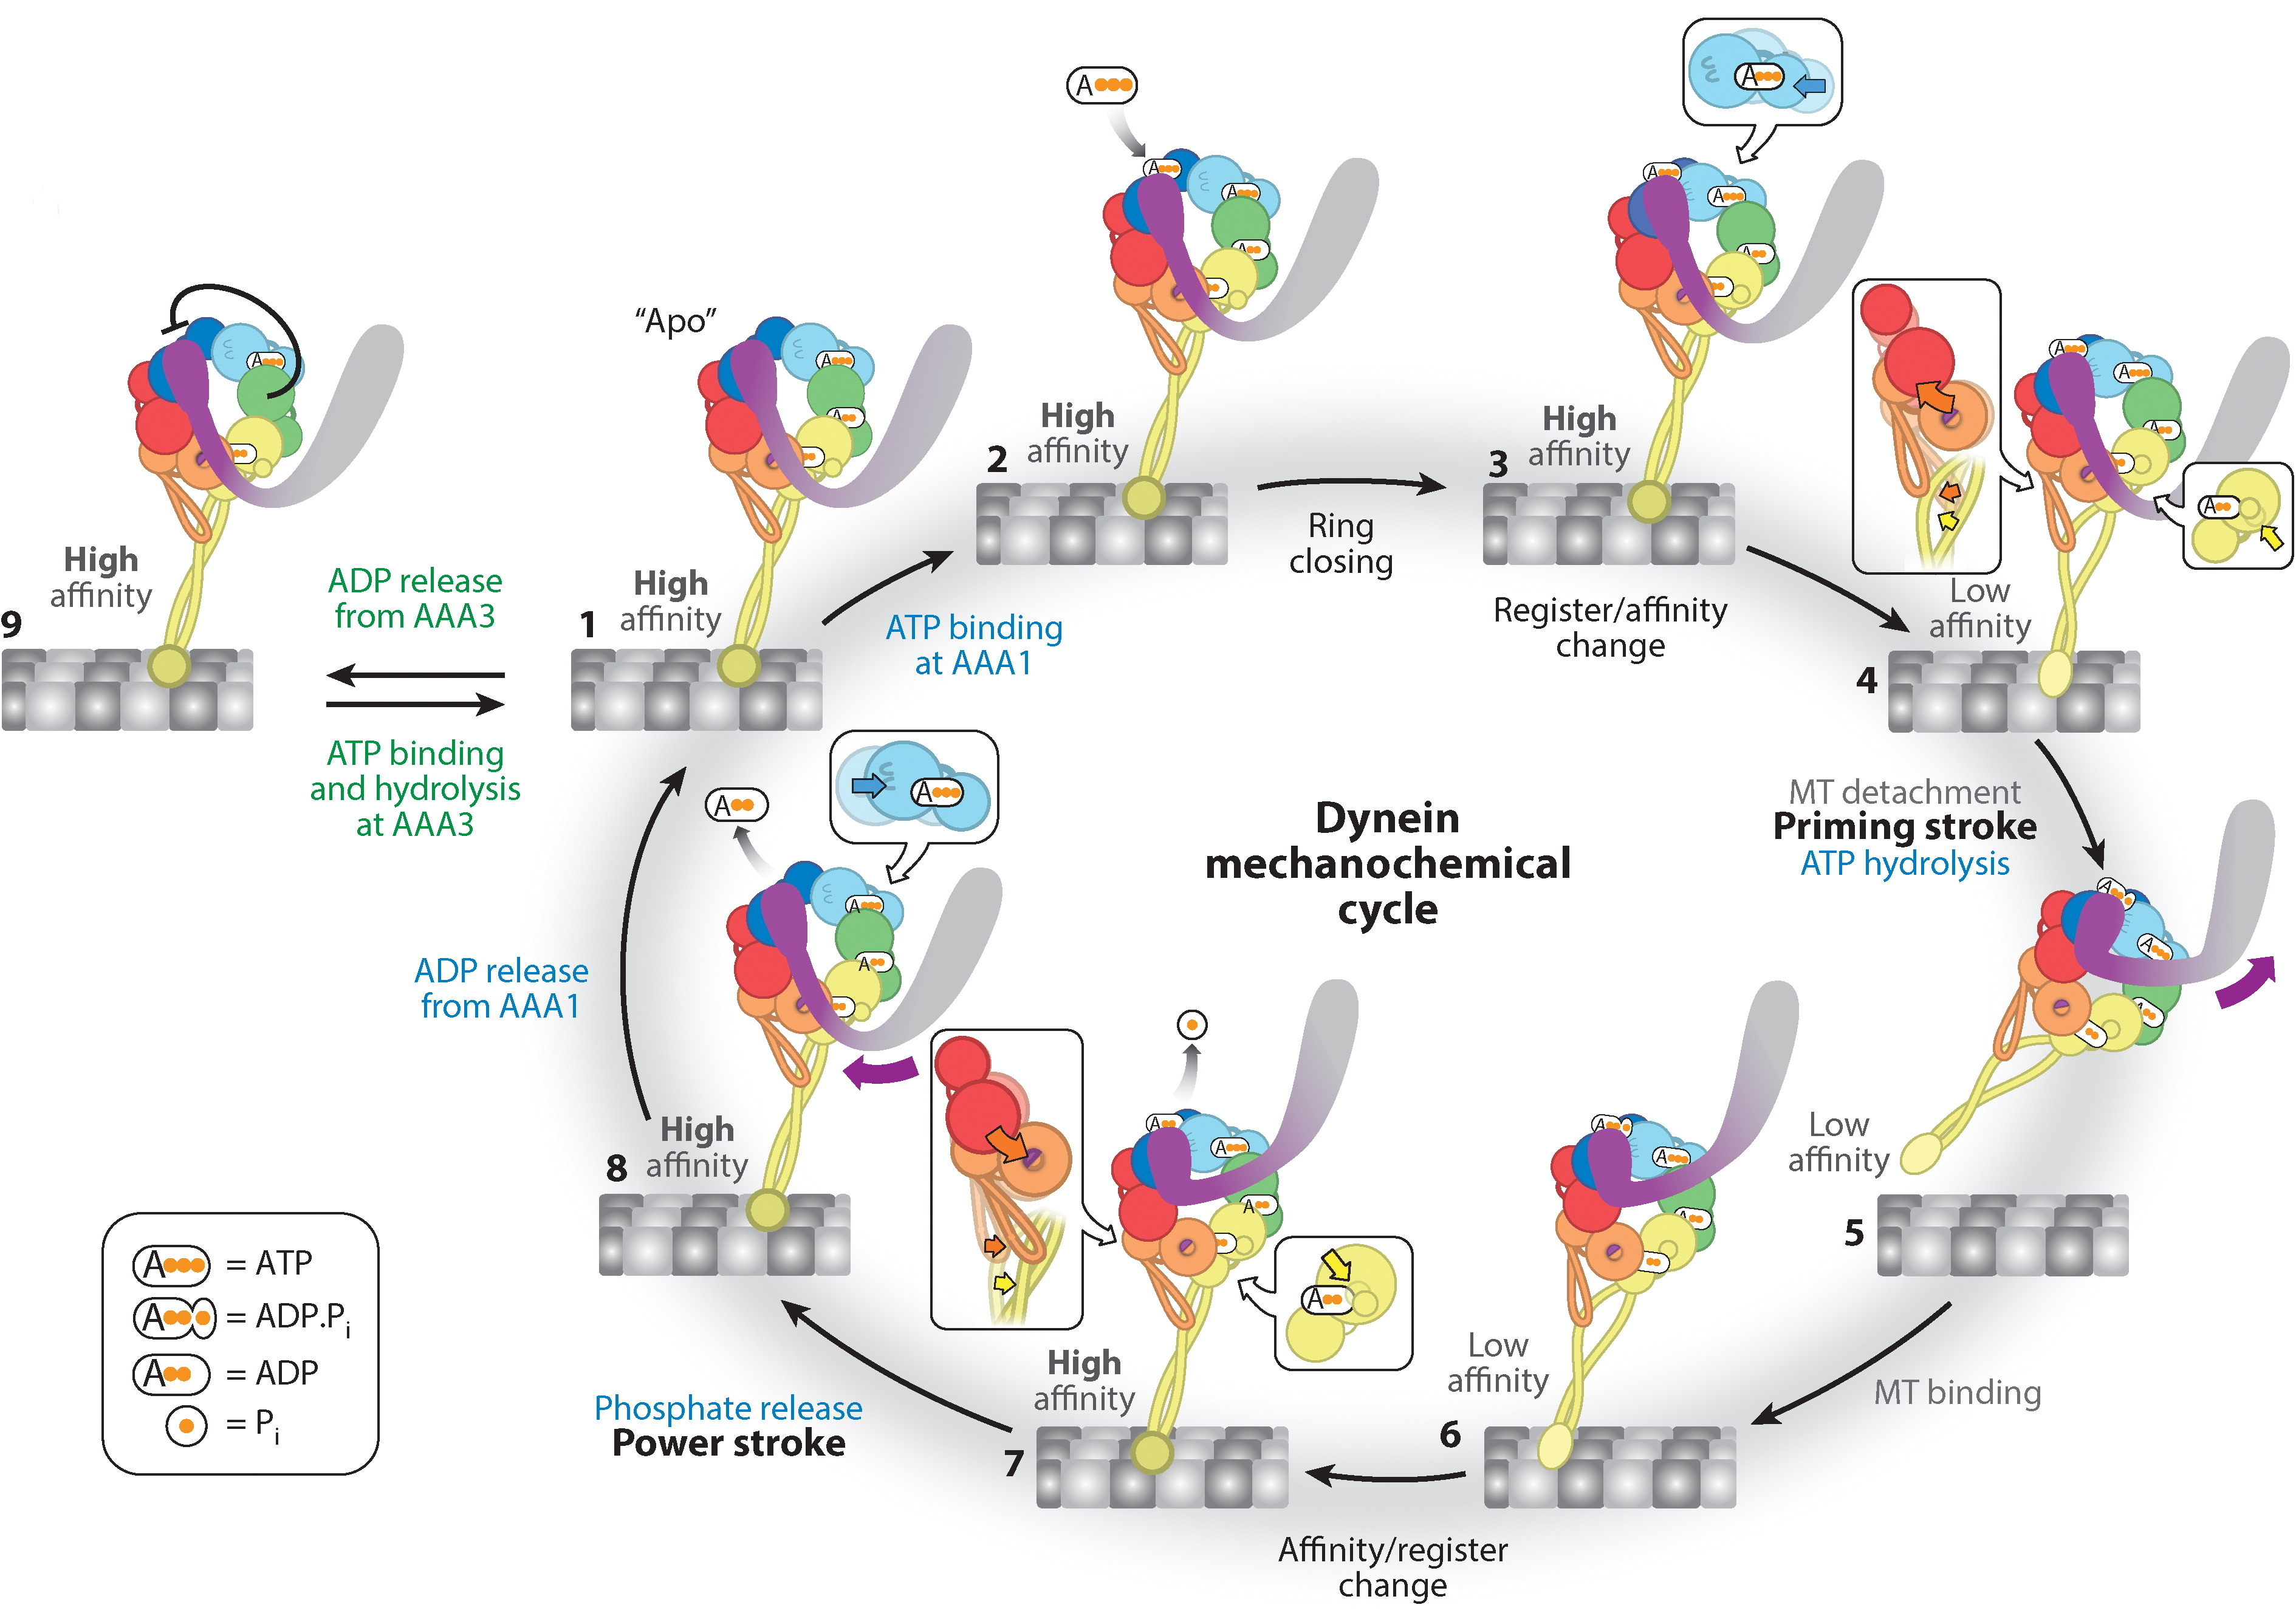
\includegraphics[width=.65\textwidth,keepaspectratio]{../figures/mechanochemical-cycle.jpeg}
  \caption{Cycle of states the dynein motor goes through during motion in the Cianfrocco model \cite{cianfroccoreview}.}
  \label{mech-cycle}
\end{figure}

\subsubsection{ATP binding / unbinding effects}
\subsubsection{Microtubule un/rebinding}
\subsubsection{Conformation change of motor (``priming stroke'')}
A FRET (fluorescent resonance energy transfer) study, which probes the closeness of different labeled domains on a protein, showed that dynein is found in two different major conformations, depending on the nucleotide bound to its AAA1 ATPase site \cite{FRETstatepaper}. When no nucleotide, ATP or ADP is bound, the authors label the protein ``state I.'' When ADP-Pi bound, the motor is said to be in ``state II,'' as shown in Fig \ref{nucleotide-state}. In addition, motors in the presence of the unhydrolyzable ATP analog were found in state II, indicating the transition from state I to II occurs during ATP binding. Similar reasoning shows that the state II to I transition occurs when the protein is ADP bound. This allows the authors to create the state diagram shown in Fig \ref{nucleotide-state-diagram}.\\

%% \begin{figure}[h]
%%   \centering
%%   \includegraphics[width=.65\textwidth,keepaspectratio]{../figures/two-state-em-diagram}
%%   \caption{}
%%   \label{nuecleotide-state}
%% \end{figure}

%% \begin{figure}[h]
%%   \centering
%%   \includegraphics[width=.65\textwidth,keepaspectratio]{../figures/nucleotide-state-cycle}
%%   \caption{}
%%   \label{nucleotide-state-diagram}
%% \end{figure}

This single FRET study illustrates how the conformational aspect of the mechanochemical cycle works. Dynein begins in state I and binds ATP into its AAA1 ATPase, changing into state II by changing its stalk-tail angle to move the tail outward. ATP is then hydrolized into ADP-Pi. Pi is then ejected from the AAA1 site, leaving ADP behind. This causes the reverse state transition, moving the tail inward. When combined with microtubule affinity changes, this primitive model of the dynein cycle could explain how dynein walks.\\

\textit{It is interesting to note that the hydrolysis of ATP is not actually used to directly power the motor -- binding AMP-PMP, a nonhydrolyzable analog of ATP, can also cause the motor to change from state I to state II \cite{FRETstatepaper}. The specialness of ATP is that it can be broken down into ADP, which causes another conformation change back to state I. Thus, something something the transfer of energy from nucleotide to motor is in its shape, not in its chemistry.}\\

\textbf{more on how ATP actually causes the conformation change, if that's available. The change from an open/closed ATPase is what changes the nucleotide affinity, go into depth on that, but actual info on how ATP binding causes conformation change would be good. Something about going from a planar to nonplanar conformation?}\\

also how crystal structures are in different positions

\subsubsection{Experimental results on dynein’s step}
Weihong's figures go here.\\

\subsubsection{c What is still needed to support theory}
Where our simulation fits in. Why we need this kind of information.
There are many different things which might be important for dynein's walk which we don't take into account: springiness of tail/stalk, changes in spring constants, repulsion between the heads, multiple pre/post powerstroke conformations. We are trying to see if these things are actually important.

\subsubsection{Other theories?}
Imamula model: how it is different from Cianfrocco model, and why we chose the Cianfrocco model.\\
	\subsection{Past Simulations}
		\subsubsection{Sarlah Winch Model}
		\subsubsection{-x Other models}
	\subsection{Brownian motion}
                \subsubsection{Introduction/derivation}
                \subsubsection{Justification}

\subsection{Simulation}
Talk about why simulation is the only way to verify the mechanochemical cycle, since experiments
aren't high resolution enough to make good videos of the walk, and even if they were, in some sense
knowing that dynein behaves identically to a simple mathematical model is more informative than
a video, since there is lots of information in a video and really precise info in a simulation.\\

\textbf{Not sure where this goes:} The 'goal' of our experiment, at a very high level, is to
understand how dynein works. We can know this if we can come up with the minimum set of characteristics a physical system needs to act like dynein. This information is the same thing as knowing
``how dynein walks.'' We don't need to know all the complex dynamics of every single amino acid in
dynein, we only need to know our rough model.\\

\subsection{Our model}
Talk about what the important parts of the mechanochemical cycle from the introduction are, and how
we take those and model them.\\
\subsubsection{Rigid point model}
Talk about two things: reducing bulky circular domains to points (is this the same as unified atom
model?) with a certain drag constant based on radius, and acting like the domains are rigid in
distance from each other. Talk about why this is valid (is it? it's an assumption, David may know
more).
\subsubsection{Harmonic energies}
How we're modeling the complicated folding and adjusting of a massive protein as a harmonic
oscillator. Why this is valid. Also other approaches...what else could we have modelled it as?
\subsubsection{Two-state model}
The mechanochemical cycle has eight states. We choose two as representative because \textbf{a.)}
many of the states are identically conformationally or \textbf{b.)} the transitions happen so fast
the intermediate states don't matter. Talk about rate constants here.
\subsubsection{Limitations}
Talk about the things we \textit{don't} take into account...motor-motor interaction, 2d information,
other ATPase nucleotide state, saying certain mechanochemical steps occur ``fast,'' not taking into
account all mechanochemical cycle states, making the coiled coil domain rigid even though it may be
springy...

Mention the Burgess paper, which says spring constants might change between apo/ADP states.

\paragraph{Euler’s method}
Show how Euler's method is arrived at, how its error scales, why we use it.

\paragraph{Vs other methods (Runge Kutta, etc)}
Talk about why our differential equation is most conducive to Euler's method. Euler's is more
efficient -- is there a way to show how our differential equation is smooth, not jagged?

\paragraph{Gibbs energy of transition}
Do some stuff with Gibb's here? Why our energies are Gibb's and not internal energy?\\

\section{Chapter: Methods}

\subsection{Dynein Models}
In order to simulate a protein's passage through the above mechanochemical cycle, two mathematical models are needed: one for the prestroke, MTBD-detached state, and one for the poststroke, MTBD-bound state. The purpose of each model is to calculate the position and velocity of each domain at an arbitrary time.\\

\subsubsection{Prestroke onebound model}
Prestroke dynein is referred to as onebound, since one motor domain is bound to the MT in this state, and the other unbound. A spatial representation of onebound dynein is shown in Figure \ref{ob_fig}. 

\begin{figure}[h]
  \centering
  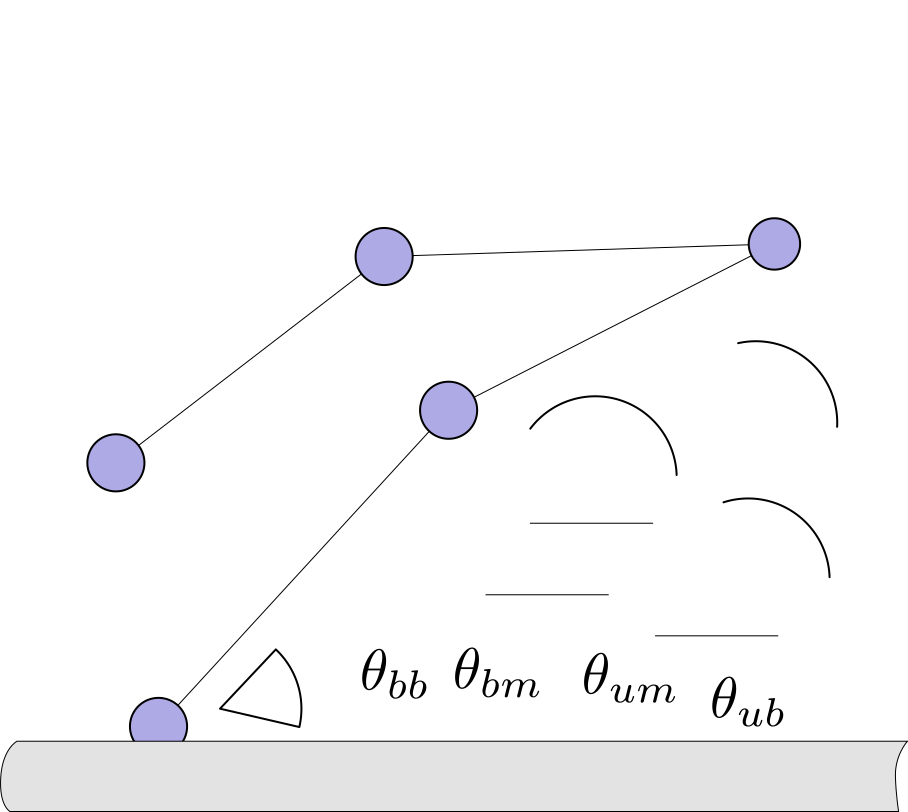
\includegraphics[width=.45\textwidth]{../figures/ob_fig.pdf}
  \caption{Definition of equilibrium angles.}
  \label{ob_fig}
\end{figure}

TODO: label domain names (MTBD motor tail), Ls, Lt, microtubule\\

Each domain is represented by a point, and is connected to other domains via fixed-length rods. Angles represent the degrees of freedom of the model. Since the protein is a dimer, there are two copies of the MTB, motor and tail domains. The tails are fused together and so represented as a single point. The motor and MTB domains are given a ``bound'' and ``unbound'' designation to differentiate them. The ``bound'' domains are the MTBD attached to the MT and its corresponding motor domain. The unbound domains are the unbound MTBD and its corresponding motor domain.\\

\paragraph{Angular and Cartesian coordinates}

The four angles $\Theta_{bb}, \Theta_{bm}, \Theta_{um}$ and $\Theta_{ub}$, corresponding to bound binding, bound motor, unbound motor and unbound binding angle, together describe any possible conformation the system can take on. The domain of $\Theta_{bb}$ has a restricted domain of $[0,\pi]$ to prevent below-MT conformations, but the other angles have domains of $[0,2\pi]$. Each angle is defined relative to the horizontal axis.\\

\begin{figure}[h]
  \centering
  \begin{tabular}{c}
    \begin{lstlisting}[language=C++]
      class Dynein_onebound{
        double &$\Theta_{bb}, \Theta_{bb}, \Theta_{bb}, \Theta_{bb}$&
        double &$\dot{\Theta}_{bb}, \dot{\Theta}_{bb}, \dot{\Theta}_{bb}, \dot{\Theta}_{bb}$&
        double &$X_{bb}$&
      }
    \end{lstlisting}
  \end{tabular}
  \caption{Pseudocode of the onebound Dynein model.}
  \label{ob_struct}
\end{figure}

Pseudocode for the numerical onebound model representation is shown in Figure \ref{ob_struct}. The position of the bound binding domain $X_{bb}$ and the four domain angles are all the values needed to determine the position of the protein at any time. The following equations allow recursive calculation of the positions of each domain in cartesian coordinates:

\noindent\begin{minipage}{0.49\linewidth}
\begin{align}
  X_{bm} &= X_{bb}+L_{s}\cos(\Theta_{bb}) \\
  X_{t}  &= X_{bm}+L_{t}\cos(\Theta_{bm}) \\
  X_{fm} &= X_{t} - L_{t}\cos(\Theta_{fm}) \\
  X_{fb} &= X_{fm} - L_{s}\cos(\Theta_{fb})
\end{align}
\end{minipage}
\begin{minipage}{0.49\linewidth}
\begin{align}
  Y_{bb} &= 0 \\
  Y_{bm} &= Y_{bb}+L_{s}\sin(\Theta_{bb}) \\
  Y_{t}  &= Y_{bm}+L_{t}\sin(\Theta_{bm}) \\
  Y_{fm} &= Y_{t} - L_{t}\sin(\Theta_{fm}) \\
  Y_{fb} &= Y_{fm} - L_{s}\sin(\Theta_{fb})
\end{align}
\end{minipage}
\vspace{.5cm}

$L_s$ and $L_t$ correspond to lengths of each interdomain rod, and the $t$ subscripts refer to tail domain coordinates.\\

\paragraph{Angular and Cartesian velocities}
The goal is to express angular velocities $\dot{\Theta}_{bb}, \dot{\Theta}_{bb}, \dot{\Theta}_{bb}$ and $\dot{\Theta}_{bb}$ in terms of known quantities. To begin, the cartesian velocities of each domain can be calculated from the above position equations in a similar recursive manner:

\noindent\begin{minipage}{0.49\linewidth}
\begin{align}
  \dot{X}_{bb} &= 0 \\
  \dot{X}_{bm} &= \dot{X}_{bb} - L_{s}\sin(\Theta_{bb})\dot{\Theta}_{bb} \label{cartesian-bmx}\\
  \dot{X}_{t } &= \dot{X}_{bm} - L_{t}\sin(\Theta_{bm})\dot{\Theta}_{bm} \\
  \dot{X}_{fm} &= \dot{X}_{t } + L_{t}\sin(\Theta_{fm})\dot{\Theta}_{fm} \\
  \dot{X}_{fb} &= \dot{X}_{fm} + L_{s}\sin(\Theta_{fb})\dot{\Theta}_{fb}
\end{align}
\end{minipage}
\begin{minipage}{0.49\linewidth}
\begin{align}                                                                          
  \dot{Y}_{bb} &= 0 \\                                                        
  \dot{Y}_{bm} &= \dot{Y}_{bb} + L_{s}\cos(\Theta_{bb})\dot{\Theta}_{bb} \\
  \dot{Y}_{t}  &= \dot{Y}_{bm} + L_{t}\cos(\Theta_{bm})\dot{\Theta}_{bm} \\
  \dot{Y}_{fm} &= \dot{Y}_{t } - L_{t}\cos(\Theta_{fm})\dot{\Theta}_{fm} \\
  \dot{Y}_{fb} &= \dot{Y}_{fm} - L_{s}\cos(\Theta_{fb})\dot{\Theta}_{fb}
\end{align}
\end{minipage}
\vspace{.5cm}

Another way to express these cartesian velocities is using the Brownian dynamics equation $\dot{X} = \frac1\gamma F_{net} + R$:

\begin{align}  
  \dot{X}_{bm} &= \frac{1}{\gamma_m} \Big(F_{xml} + - \lambda_{bs}(X_{bm} - X_{bb}) + \lambda_{bt}(X_{t } - X_{bm}) \Big) + R_{xml} \label{brownian-bmx}\\
  \dot{X}_{t } &= \frac{1}{\gamma_t} \Big(F_{xt } + - \lambda_{bt}(X_{t } - X_{bm}) + \lambda_{ft}(X_{fm} - X_{t }) \Big) + R_{xt } \\
  \dot{X}_{fm} &= \frac{1}{\gamma_m} \Big(F_{xmr} + - \lambda_{ft}(X_{fm} - X_{t }) + \lambda_{fs}(X_{fb} - X_{fm}) \Big) + R_{xmr} \\
  \dot{X}_{fb} &= \frac{1}{\gamma_b} \Big(F_{xbr} + - \lambda_{fs}(X_{fb} - X_{fm}) \Big) + R_{xbr}
\end{align}

\begin{align}  
  \dot{Y}_{bm} &= \frac{1}{\gamma_m} \Big(F_{yml} + - \lambda_{bs}(Y_{bm} - Y_{bb}) + \lambda_{bt}(Y_{t } - Y_{bm}) \Big) + R_{yml} \\
  \dot{Y}_{t}  &= \frac{1}{\gamma_t} \Big(F_{yt } + - \lambda_{bt}(Y_{t } - Y_{bm}) + \lambda_{ft}(Y_{fm} - Y_{t }) \Big) + R_{yt } \\
  \dot{Y}_{fm} &= \frac{1}{\gamma_m} \Big(F_{ymr} + - \lambda_{ft}(Y_{fm} - Y_{t }) + \lambda_{fs}(Y_{fb} - Y_{fm}) \Big) + R_{ymr} \\
  \dot{Y}_{fb} &= \frac{1}{\gamma_b} \Big(F_{ybr} + - \lambda_{fs}(Y_{fb} - Y_{fm}) \Big) + R_{ybr}
\end{align}

where $\gamma_n$ is a drag coefficient for the binding, motor or tail domain with units of mass per second. $F_{xn}$ is the x component of external force on each domain $n$ due to various factors. $\lambda_{12}\left(X_1 - X_2\right)$ is the x component of internal force on domain $2$ due to domain $1$, where $\lambda$ is a tension coefficient with units of mass per second per second. $R_{xn}$ is the Brownian coefficient representing motion due to solvent collision, with units of velocity.\\

These two sets of equations, cartesian and Brownian, can be equated to get more interesting equations. For example, Eq (\ref{cartesian-bmx}) and Eq (\ref{brownian-bmx}) can be equated. This equating, combined with expanding the recursive velocity definitions leads to: 

\begin{align*}
  -L_s\sin(\theta_{bb})\dot{\theta}_{bb} &= \frac{1}{\gamma_m}F_{xml} + -\frac{1}{\gamma_m}\lambda_{bs}(X_{bm} - X_{bb}) + \frac{1}{\gamma_m}\lambda_{bt}(X_{t } - X_{bm}) + R_{bmx} \\
  -L_s\sin(\theta_{bb})\dot{\theta}_{bb} - L_t\sin(\theta_{bm})\dot{\theta}_{bm} &= \frac{1}{\gamma_t}F_{xt } + -\frac{1}{\gamma_t}\lambda_{bt}(X_{t } - X_{bm}) + \frac{1}{\gamma_t}\lambda_{ft}(X_{um} - X_{t }) + R_{tx} \\
  -L_s\sin(\theta_{bb})\dot{\theta}_{bb} - L_t\sin(\theta_{bm})\dot{\theta}_{bm} + L_t\sin(\theta_{um})\dot{\theta}_{um} &= \frac{1}{\gamma_m}F_{xmr} + -\frac{1}{\gamma_m}\lambda_{ft}(X_{um} - X_{t }) + \frac{1}{\gamma_m}\lambda_{fs}(X_{ub} - X_{um}) + R_{bmx} \\
  -L_s\sin(\theta_{bb})\dot{\theta}_{bb} - L_t\sin(\theta_{bm})\dot{\theta}_{bm} + L_t\sin(\theta_{um})\dot{\theta}_{um} + L_s\sin(\theta_{ub})\dot{\theta}_{ub} &= \frac{1}{\gamma_b}F_{xbr} + -\frac{1}{\gamma_b}\lambda_{fs}(X_{ub} - X_{um}) + R_{bbx}
\end{align*}

\begin{align*}
  L_s\cos(\theta_{bb})\dot{\theta}_{bm} &= \frac{1}{\gamma_m}F_{yml} + -\frac{1}{\gamma_m}\lambda_{bs}(Y_{bm} - Y_{bb}) + \frac{1}{\gamma_m}\lambda_{bt}(Y_{t } - Y_{bm}) + R_{umy} \\
  L_s\cos(\theta_{bb})\dot{\theta}_{bb} + L_t\cos(\theta_{bm})\dot{\theta}_{bm} &= \frac{1}{\gamma_t}F_{yt } + -\frac{1}{\gamma_t}\lambda_{bt}(Y_{t } - Y_{bm}) + \frac{1}{\gamma_t}\lambda_{ft}(Y_{um} - Y_{t }) + R_{ty} \\
  L_s\cos(\theta_{bb})\dot{\theta}_{bb} + L_t\cos(\theta_{bm})\dot{\theta}_{bm} - L_t\cos(\theta_{um})\dot{\theta}_{um} &= \frac{1}{\gamma_m}F_{ymr} + -\frac{1}{\gamma_m}\lambda_{ft}(Y_{um} - Y_{t }) + \frac{1}{\gamma_m}\lambda_{fs}(Y_{ub} - Y_{um}) + R_{bmy} \\
  L_s\cos(\theta_{bb})\dot{\theta}_{bb} + L_t\cos(\theta_{bm})\dot{\theta}_{bm} - L_t\cos(\theta_{um})\dot{\theta}_{um} - L_s\cos(\theta_{ub})\dot{\theta}_{ub} &= \frac{1}{\gamma_b}F_{ybr} + -\frac{1}{\gamma_b}\lambda_{fs}(Y_{ub} - Y_{um}) + R_{bby}
\end{align*}

These eight equations form a system of equations with eight unknowns: $\dot{\Theta}_{bb}, \dot{\Theta}_{bb}, \dot{\Theta}_{bb}$ and $\dot{\Theta}_{bb}$, and the four tension coefficients $\lambda_{bs}, \lambda_{bt}, \lambda_{um}$ and $\lambda_{ub}$. This system is more compactly represented as:
{\small
  \[
  \hspace{-1.0cm}
  \resizebox{0.85\linewidth}{!}{%
  $\begin{pmatrix}
    L_s\sin\theta_{bb} & 0 & 0 & 0 & -\gamma_m (X_{bm} - X_{bb}) & \gamma_m (X_{t } - X_{bm}) & 0 & 0\\
    L_s\sin(\theta_{bb}) & L_t\sin(\theta_{bm}) & 0 & 0 & 0 & -\gamma_t (X_{t } - X_{bm}) & \gamma_t (X_{um} - X_{t }) & 0\\
    L_s\sin(\theta_{bb}) & L_t\sin(\theta_{bm}) & -L_t\sin(\theta_{um}) & 0 & 0 & 0 & -\gamma_m (X_{um} - X_{t }) & \gamma_m (X_{ub} - X_{um})\\
    L_s\sin(\theta_{bb}) & L_t\sin(\theta_{bm}) & -L_t\sin(\theta_{um}) & -L_s\sin(\theta_{ub}) & 0 & 0 & 0 & -\gamma_b (X_{ub} - X_{um})\\
    -L_s\cos(\theta_{bb}) & 0 & 0 & 0 & -\gamma_m (Y_{bm} - Y_{bb}) & \gamma_m (Y_{t } - Y_{bm}) & 0 & 0\\
    -L_s\cos(\theta_{bb}) & -L_t\cos(\theta_{bm}) & 0 & 0 & 0 & -\gamma_t (Y_{t } - Y_{bm}) & \gamma_t (Y_{um} - Y_{t }) & 0\\
    -L_s\cos(\theta_{bb}) & -L_t\cos(\theta_{bm}) & L_t\cos(\theta_{um}) & 0 & 0 & 0 & -\gamma_m (Y_{um} - Y_{t }) & \gamma_m (Y_{ub} - Y_{um})\\
    -L_s\cos(\theta_{bb}) & -L_t\cos(\theta_{bm}) & L_t\cos(\theta_{um}) & L_s\cos(\theta_{ub}) & 0 & 0 & 0 & -\gamma_b (Y_{ub} - Y_{um})\\
  \end{pmatrix}$%
  }
  \begin{pmatrix}
    \dot{\theta}_{bb}\\
    \dot{\theta}_{bm}\\
    \dot{\theta}_{um}\\
    \dot{\theta}_{ub}\\
    \lambda_{bs}\\
    \lambda_{bt}\\
    \lambda_{ut}\\
    \lambda_{us}\\
  \end{pmatrix}
  =
  \begin{pmatrix}
    -F_{bmx} + \gamma_m R_{bmx}\\
    -F_{tx} + \gamma_t R_{tx}\\
    -F_{umx} + \gamma_m R_{umx}\\
    -F_{ubx} + \gamma_b R_{ubx}\\
    -F_{bmy} + \gamma_m R_{bmy}\\
    -F_{ty} + \gamma_t R_{ty}\\
    -F_{umy} + \gamma_m R_{umy}\\
    -F_{uby} + \gamma_b R_{uby}\\
  \end{pmatrix}
  \]
}

This matrix is then solved using the Mathematica algebra system, resulting in a set of equations shown in Appendix (\ref{ob-motion-equations]}).

------------------------------------------

\begin{figure}[h!]
  \centering
  \begin{minipage}[b]{0.49\textwidth}
    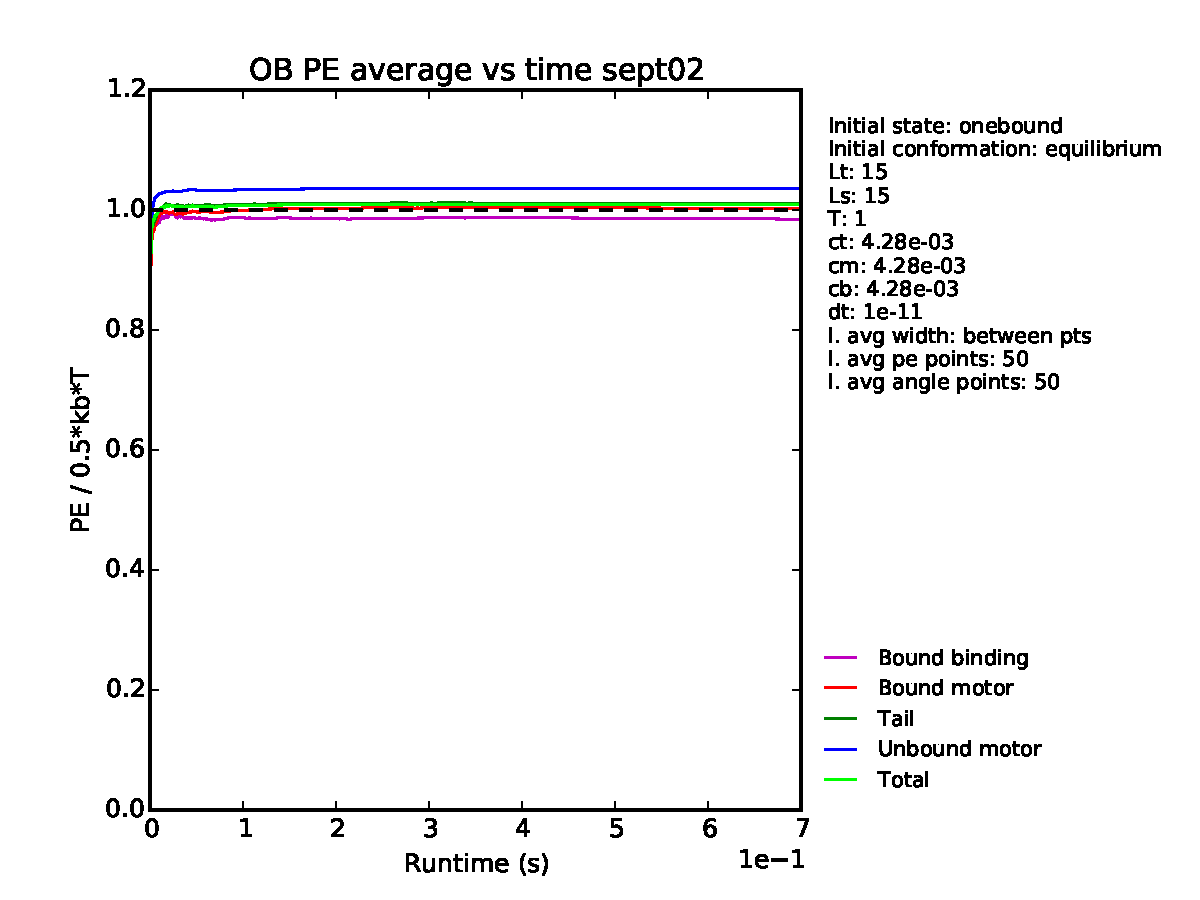
\includegraphics[width=\textwidth]{../figures/OB_Average_PE.pdf}
    \caption{Onebound PE vs time.}
  \end{minipage}
  \begin{minipage}[b]{0.49\textwidth}
    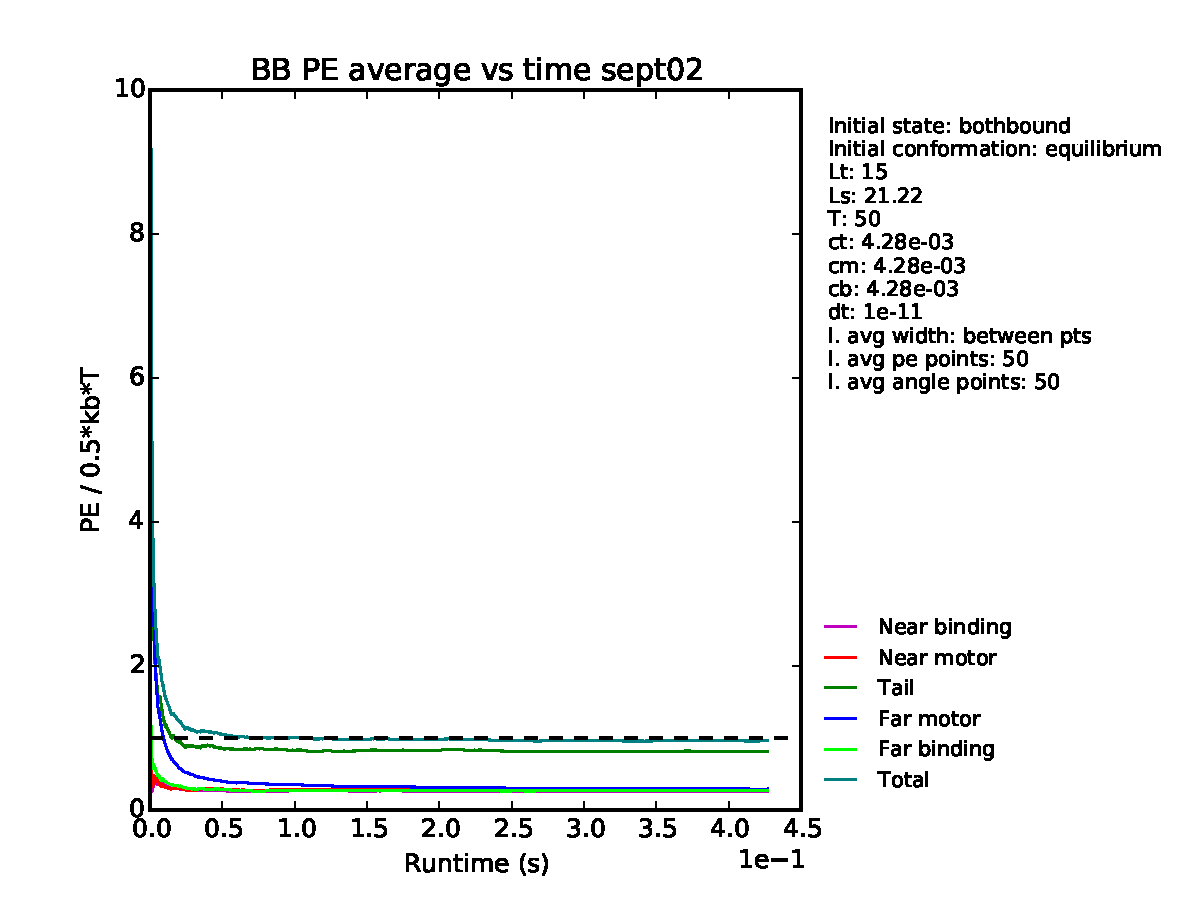
\includegraphics[width=\textwidth]{../figures/BB_Average_PE.pdf}
    \caption{Bothbound PE vs time.}
  \end{minipage}
  \label{fig:equipartition_agreement}
\end{figure}


\section{Chapter: Results}
	\subsection{Histograms}
		\subsubsection{Step length histograms}
		\subsubsection{Step time histograms}
	\subsection{Other ways to represent data?}

\section{Chapter: Discussion}
\subsection{Why our model worked, didn’t work}
Fill this out over winter when you know more.\\
\subsection{Future work on this project}
If setbacks happen, this'll be a big section. Or, further simulations which could be done.

\subsubsection{Experiments to verify our model}
Talk about how FRET could be used to verify our model. We have domain distance info over long
timescales in our model - this is something we could compare to a FRET experiment exploring
the distance between domains in dynein.\\

Other biophysics experiments which could verify our model?\\

Do our spring constants seem to indicate that the protein does about one ATP's worth of work through its cycle? I wonder if the motor cools down its surroundings when it walks...\\

Calorimetry could get Gibb's energy of binding if you froze the motor in onebound using
vanadium? Maybe...\\
\subsection{Possible further projects}
\subsection{Difference between dynein and kinesin}
Our project un/successfully predicted how dynein behaved. How would we modify it to describe kinesin?
Is dynein's linker-motor connection less tense than kinesin's, leading to more random motion? This
would likely be lots of speculation, but it could be cool to look up some papers on kinesin motility
and get its crystal structure to do some comparisons.

\bibliography{thesis-articles}

%% \bibliography{thesis-webpages}

\section{Appendix}

\subsection{Motion equations}

\subsubsection{Onebound equations}
\label{onebound-motion-equations}
These are the full motion equations used to time-evolve the onebound model:

\begin{align*}
AA &= L_s\sin\theta_{bb}      &   LL &= -L_s\cos(\theta_{bb})\\
BB &= L_t\sin(\theta_{bm})    &	 MM &= -L_t\cos(\theta_{bm})\\
CC &= -L_t\sin(\theta_{um})   &	 NN &= L_t\cos(\theta_{um})\\
DD &= -L_s\sin(\theta_{ub})   &	 OO &= L_s\cos(\theta_{ub})\\
\\
EE &= -\gamma_m (X_{bm} - X_{bb})       &  PP &= -\gamma_m (Y_{bm} - Y_{bb})\\
FF &= \gamma_m (X_{t } - X_{bm})        &	 QQ &= \gamma_m (Y_{t } - Y_{bm})\\ 
GG &= -\gamma_t (X_{t } - X_{bm})       &	 RR &= -\gamma_t (Y_{t } - Y_{bm})\\
HH &= \gamma_t (X_{um} - X_{t })        &	 SS &= \gamma_t (Y_{um} - Y_{t })\\ 
II &= -\gamma_m (X_{um} - X_{t })       &	 TT &= -\gamma_m (Y_{um} - Y_{t })\\
JJ &= \gamma_m (X_{ub} - X_{um})        &	 UU &= \gamma_m (Y_{ub} - Y_{um})\\ 
KK &= -\gamma_b (X_{ub} - X_{um})       &	 VV &= -\gamma_b (Y_{ub} - Y_{um})\\
\end{align*}%
%
\[
\begin{pmatrix}
  AA & 0 & 0 & 0 & EE & FF & 0 & 0\\
  AA & BB & 0 & 0 & 0 & GG & HH & 0\\
  AA & BB & CC & 0 & 0 & 0 & II & JJ\\
  AA & BB & CC & DD & 0 & 0 & 0 & KK\\
  LL & 0 & 0 & 0 & PP & QQ & 0 & 0\\
  LL & MM & 0 & 0 & 0 & RR & SS & 0\\
  LL & MM & NN & 0 & 0 & 0 & TT & UU\\
  LL & MM & NN & OO & 0 & 0 & 0 & VV\\
\end{pmatrix}
\begin{pmatrix}
    \dot{\theta}_{bb}\\
    \dot{\theta}_{bm}\\
    \dot{\theta}_{um}\\
    \dot{\theta}_{ub}\\
    \lambda_{bs}\\
    \lambda_{bt}\\
    \lambda_{ut}\\
    \lambda_{us}\\
  \end{pmatrix}
=
\begin{pmatrix}
  X1\\
  X2\\
  X3\\
  X4\\
  X5\\
  X6\\
  X7\\
  X8\\
\end{pmatrix}
\]

Solving the above system for $\dot{\Theta}_{bb}, \dot{\Theta}_{bb}, \dot{\Theta}_{bb}$ and $\dot{\Theta}_{bb}$ gives

\begin{multline}
d_bba = (-(GG*II*MM*NN*PP*X1) + CC*HH*MM*PP*RR*X1 -
      BB*HH*NN*PP*RR*X1 + BB*II*NN*PP*RR*X1 - CC*GG*MM*PP*SS*X1 +
      BB*GG*NN*PP*SS*X1 + CC*GG*MM*PP*TT*X1 - BB*CC*PP*RR*TT*X1 +
      FF*II*MM*NN*PP*X2 - EE*II*MM*NN*QQ*X2 + CC*FF*MM*PP*SS*X2 -
      BB*FF*NN*PP*SS*X2 - CC*EE*MM*QQ*SS*X2 + BB*EE*NN*QQ*SS*X2 -
      CC*FF*MM*PP*TT*X2 + CC*EE*MM*QQ*TT*X2 - FF*HH*MM*NN*PP*X3 +
      EE*HH*MM*NN*QQ*X3 + BB*FF*NN*PP*SS*X3 - BB*EE*NN*QQ*SS*X3 +
      EE*GG*II*MM*NN*X5 - CC*EE*HH*MM*RR*X5 + BB*EE*HH*NN*RR*X5 -
      BB*EE*II*NN*RR*X5 + CC*EE*GG*MM*SS*X5 - BB*EE*GG*NN*SS*X5 -
      CC*EE*GG*MM*TT*X5 + BB*CC*EE*RR*TT*X5 - CC*FF*HH*MM*PP*X6 +
      BB*FF*HH*NN*PP*X6 - BB*FF*II*NN*PP*X6 + CC*EE*HH*MM*QQ*X6 -
      BB*EE*HH*NN*QQ*X6 + BB*EE*II*NN*QQ*X6 + BB*CC*FF*PP*TT*X6 -
      BB*CC*EE*QQ*TT*X6 + CC*FF*HH*MM*PP*X7 - CC*EE*HH*MM*QQ*X7 -
      BB*CC*FF*PP*SS*X7 + BB*CC*EE*QQ*SS*X7)/ (EE*GG*II*LL*MM*NN +
      BB*FF*HH*LL*NN*PP - BB*FF*II*LL*NN*PP - AA*FF*HH*MM*NN*PP +
      AA*FF*II*MM*NN*PP - AA*GG*II*MM*NN*PP - BB*EE*HH*LL*NN*QQ +
      BB*EE*II*LL*NN*QQ + AA*EE*HH*MM*NN*QQ - AA*EE*II*MM*NN*QQ -
      CC*EE*HH*LL*MM*RR + BB*EE*HH*LL*NN*RR - BB*EE*II*LL*NN*RR +
      AA*CC*HH*MM*PP*RR - AA*BB*HH*NN*PP*RR + AA*BB*II*NN*PP*RR +
      CC*EE*GG*LL*MM*SS - BB*EE*GG*LL*NN*SS - BB*CC*FF*LL*PP*SS +
      AA*CC*FF*MM*PP*SS - AA*CC*GG*MM*PP*SS + AA*BB*GG*NN*PP*SS +
      BB*CC*EE*LL*QQ*SS - AA*CC*EE*MM*QQ*SS - CC*EE*GG*LL*MM*TT +
      BB*CC*FF*LL*PP*TT - AA*CC*FF*MM*PP*TT + AA*CC*GG*MM*PP*TT -
      BB*CC*EE*LL*QQ*TT + AA*CC*EE*MM*QQ*TT + BB*CC*EE*LL*RR*TT -
      AA*BB*CC*PP*RR*TT) - ((FF*PP - EE*QQ)*(HH*MM - BB*SS)*(JJ*NN -
      CC*UU)*(-(((Power(AA,6)*Power(BB,2)*CC*DD*HH*MM -
      Power(AA,6)*Power(BB,3)*DD*HH*NN +
      Power(AA,6)*Power(BB,3)*DD*II*NN -
      Power(AA,6)*Power(BB,3)*CC*II*OO)* (-(EE*LL) +
      AA*PP)*(-((Power(AA,3)*Power(BB,2)*CC*EE*LL -
      Power(AA,4)*BB*CC*EE*MM)*(-(FF*LL) + AA*QQ)) + (-(EE*LL) +
      AA*PP)*(Power(AA,4)*BB*CC*GG*MM -
      Power(AA,2)*BB*CC*(-(AA*BB*FF*LL) + Power(AA,2)*FF*MM +
      Power(AA,2)*BB*RR))) - (-(EE*LL) +
      AA*PP)*((Power(AA,5)*Power(BB,3)*CC*DD*FF*LL -
      Power(AA,6)*Power(BB,2)*CC*DD*FF*MM +
      Power(AA,6)*Power(BB,2)*CC*DD*GG*MM -
      Power(AA,6)*Power(BB,3)*DD*GG*NN)* (-(EE*LL) + AA*PP) -
      (Power(AA,5)*Power(BB,3)*CC*DD*EE*LL -
      Power(AA,6)*Power(BB,2)*CC*DD*EE*MM)*(-(FF*LL) +
      AA*QQ))*(Power(AA,4)*BB*CC*HH*MM -
      Power(AA,4)*Power(BB,2)*CC*SS))*
      (-(((Power(AA,3)*Power(BB,2)*CC*FF*LL - Power(AA,4)*BB*CC*FF*MM
      + Power(AA,4)*BB*CC*GG*MM -
      Power(AA,4)*Power(BB,2)*GG*NN)*(-(EE*LL) + AA*PP) -
      (Power(AA,3)*Power(BB,2)*CC*EE*LL -
      Power(AA,4)*BB*CC*EE*MM)*(-(FF*LL) + AA*QQ))*
      (-((Power(AA,3)*Power(BB,2)*CC*EE*LL -
      Power(AA,4)*BB*CC*EE*MM)*(-(LL*X1) + AA*X5)) + (-(EE*LL) +
      AA*PP)*(Power(AA,3)*Power(BB,2)*CC*LL*X1 -
      Power(AA,4)*BB*CC*MM*X1 + Power(AA,4)*BB*CC*MM*X2 -
      Power(AA,4)*Power(BB,2)*CC*X6))) +
      (-((Power(AA,3)*Power(BB,2)*CC*EE*LL -
      Power(AA,4)*BB*CC*EE*MM)*(-(FF*LL) + AA*QQ)) + (-(EE*LL) +
      AA*PP)*(Power(AA,4)*BB*CC*GG*MM -
      Power(AA,2)*BB*CC*(-(AA*BB*FF*LL) + Power(AA,2)*FF*MM +
      Power(AA,2)*BB*RR)))* (-((Power(AA,3)*Power(BB,2)*CC*EE*LL -
      Power(AA,4)*BB*CC*EE*MM)*(-(LL*X1) + AA*X5)) + (-(EE*LL) +
      AA*PP)*(Power(AA,3)*Power(BB,2)*CC*LL*X1 -
      Power(AA,4)*BB*CC*MM*X1 + Power(AA,4)*BB*CC*MM*X2 -
      Power(AA,4)*Power(BB,2)*NN*X2 + Power(AA,4)*Power(BB,2)*NN*X3 -
      Power(AA,4)*Power(BB,2)*CC*X7)))) + (-((-(EE*LL) +
      AA*PP)*((Power(AA,3)*Power(BB,2)*CC*FF*LL -
      Power(AA,4)*BB*CC*FF*MM + Power(AA,4)*BB*CC*GG*MM -
      Power(AA,4)*Power(BB,2)*GG*NN)* (-(EE*LL) + AA*PP) -
      (Power(AA,3)*Power(BB,2)*CC*EE*LL -
      Power(AA,4)*BB*CC*EE*MM)*(-(FF*LL) +
      AA*QQ))*(Power(AA,4)*BB*CC*HH*MM -
      Power(AA,4)*Power(BB,2)*CC*SS)) + (-(EE*LL) +
      AA*PP)*(-((Power(AA,3)*Power(BB,2)*CC*EE*LL -
      Power(AA,4)*BB*CC*EE*MM)*(-(FF*LL) + AA*QQ)) + (-(EE*LL) +
      AA*PP)*(Power(AA,4)*BB*CC*GG*MM -
      Power(AA,2)*BB*CC*(-(AA*BB*FF*LL) + Power(AA,2)*FF*MM +
      Power(AA,2)*BB*RR)))* (Power(AA,4)*BB*CC*HH*MM -
      Power(AA,4)*Power(BB,2)*HH*NN + Power(AA,4)*Power(BB,2)*II*NN -
      Power(AA,4)*Power(BB,2)*CC*TT))*
      (-(((Power(AA,5)*Power(BB,3)*CC*DD*FF*LL -
      Power(AA,6)*Power(BB,2)*CC*DD*FF*MM +
      Power(AA,6)*Power(BB,2)*CC*DD*GG*MM -
      Power(AA,6)*Power(BB,3)*DD*GG*NN)*(-(EE*LL) + AA*PP) -
      (Power(AA,5)*Power(BB,3)*CC*DD*EE*LL -
      Power(AA,6)*Power(BB,2)*CC*DD*EE*MM)*(-(FF*LL) + AA*QQ))*
      (-((Power(AA,3)*Power(BB,2)*CC*EE*LL -
      Power(AA,4)*BB*CC*EE*MM)*(-(LL*X1) + AA*X5)) + (-(EE*LL) +
      AA*PP)*(Power(AA,3)*Power(BB,2)*CC*LL*X1 -
      Power(AA,4)*BB*CC*MM*X1 + Power(AA,4)*BB*CC*MM*X2 -
      Power(AA,4)*Power(BB,2)*CC*X6))) +
      (-((Power(AA,3)*Power(BB,2)*CC*EE*LL -
      Power(AA,4)*BB*CC*EE*MM)*(-(FF*LL) + AA*QQ)) + (-(EE*LL) +
      AA*PP)*(Power(AA,4)*BB*CC*GG*MM -
      Power(AA,2)*BB*CC*(-(AA*BB*FF*LL) + Power(AA,2)*FF*MM +
      Power(AA,2)*BB*RR)))* (-((Power(AA,5)*Power(BB,3)*CC*DD*EE*LL -
      Power(AA,6)*Power(BB,2)*CC*DD*EE*MM)*(-(LL*X1) + AA*X5)) +
      (-(EE*LL) + AA*PP)*(Power(AA,5)*Power(BB,3)*CC*DD*LL*X1 -
      Power(AA,6)*Power(BB,2)*CC*DD*MM*X1 +
      Power(AA,6)*Power(BB,2)*CC*DD*MM*X2 -
      Power(AA,6)*Power(BB,3)*DD*NN*X2 +
      Power(AA,6)*Power(BB,3)*DD*NN*X3 -
      Power(AA,6)*Power(BB,3)*CC*OO*X3 +
      Power(AA,6)*Power(BB,3)*CC*OO*X4 -
      Power(AA,6)*Power(BB,3)*CC*DD*X8)))))/ ((-(EE*GG*II*LL*MM*NN) -
      BB*FF*HH*LL*NN*PP + BB*FF*II*LL*NN*PP + AA*FF*HH*MM*NN*PP -
      AA*FF*II*MM*NN*PP + AA*GG*II*MM*NN*PP + BB*EE*HH*LL*NN*QQ -
      BB*EE*II*LL*NN*QQ - AA*EE*HH*MM*NN*QQ + AA*EE*II*MM*NN*QQ +
      CC*EE*HH*LL*MM*RR - BB*EE*HH*LL*NN*RR + BB*EE*II*LL*NN*RR -
      AA*CC*HH*MM*PP*RR + AA*BB*HH*NN*PP*RR - AA*BB*II*NN*PP*RR -
      CC*EE*GG*LL*MM*SS + BB*EE*GG*LL*NN*SS + BB*CC*FF*LL*PP*SS -
      AA*CC*FF*MM*PP*SS + AA*CC*GG*MM*PP*SS - AA*BB*GG*NN*PP*SS -
      BB*CC*EE*LL*QQ*SS + AA*CC*EE*MM*QQ*SS + CC*EE*GG*LL*MM*TT -
      BB*CC*FF*LL*PP*TT + AA*CC*FF*MM*PP*TT - AA*CC*GG*MM*PP*TT +
      BB*CC*EE*LL*QQ*TT - AA*CC*EE*MM*QQ*TT - BB*CC*EE*LL*RR*TT +
      AA*BB*CC*PP*RR*TT)* (-((-(EE*LL) +
      AA*PP)*(-((Power(AA,3)*Power(BB,2)*CC*EE*LL -
      Power(AA,4)*BB*CC*EE*MM)*(-(FF*LL) + AA*QQ)) + (-(EE*LL) +
      AA*PP)*(Power(AA,4)*BB*CC*GG*MM -
      Power(AA,2)*BB*CC*(-(AA*BB*FF*LL) + Power(AA,2)*FF*MM +
      Power(AA,2)*BB*RR)))* ((Power(AA,6)*Power(BB,2)*CC*DD*HH*MM -
      Power(AA,6)*Power(BB,3)*DD*HH*NN +
      Power(AA,6)*Power(BB,3)*DD*II*NN -
      Power(AA,6)*Power(BB,3)*CC*II*OO)*(-(EE*LL) + AA*PP)*
      (-((Power(AA,3)*Power(BB,2)*CC*EE*LL -
      Power(AA,4)*BB*CC*EE*MM)*(-(FF*LL) + AA*QQ)) + (-(EE*LL) +
      AA*PP)*(Power(AA,4)*BB*CC*GG*MM -
      Power(AA,2)*BB*CC*(-(AA*BB*FF*LL) + Power(AA,2)*FF*MM +
      Power(AA,2)*BB*RR))) - (-(EE*LL) +
      AA*PP)*((Power(AA,5)*Power(BB,3)*CC*DD*FF*LL -
      Power(AA,6)*Power(BB,2)*CC*DD*FF*MM +
      Power(AA,6)*Power(BB,2)*CC*DD*GG*MM -
      Power(AA,6)*Power(BB,3)*DD*GG*NN)* (-(EE*LL) + AA*PP) -
      (Power(AA,5)*Power(BB,3)*CC*DD*EE*LL -
      Power(AA,6)*Power(BB,2)*CC*DD*EE*MM)*(-(FF*LL) +
      AA*QQ))*(Power(AA,4)*BB*CC*HH*MM -
      Power(AA,4)*Power(BB,2)*CC*SS))* (Power(AA,4)*Power(BB,2)*JJ*NN
      - Power(AA,4)*Power(BB,2)*CC*UU)) + (-(EE*LL) + AA*PP)*
      (-((Power(AA,3)*Power(BB,2)*CC*EE*LL -
      Power(AA,4)*BB*CC*EE*MM)*(-(FF*LL) + AA*QQ)) + (-(EE*LL) +
      AA*PP)*(Power(AA,4)*BB*CC*GG*MM -
      Power(AA,2)*BB*CC*(-(AA*BB*FF*LL) + Power(AA,2)*FF*MM +
      Power(AA,2)*BB*RR)))* (-((-(EE*LL) +
      AA*PP)*((Power(AA,3)*Power(BB,2)*CC*FF*LL -
      Power(AA,4)*BB*CC*FF*MM + Power(AA,4)*BB*CC*GG*MM -
      Power(AA,4)*Power(BB,2)*GG*NN)*(-(EE*LL) + AA*PP) -
      (Power(AA,3)*Power(BB,2)*CC*EE*LL -
      Power(AA,4)*BB*CC*EE*MM)*(-(FF*LL) +
      AA*QQ))*(Power(AA,4)*BB*CC*HH*MM -
      Power(AA,4)*Power(BB,2)*CC*SS)) + (-(EE*LL) +
      AA*PP)*(-((Power(AA,3)*Power(BB,2)*CC*EE*LL -
      Power(AA,4)*BB*CC*EE*MM)*(-(FF*LL) + AA*QQ)) + (-(EE*LL) +
      AA*PP)*(Power(AA,4)*BB*CC*GG*MM -
      Power(AA,2)*BB*CC*(-(AA*BB*FF*LL) + Power(AA,2)*FF*MM +
      Power(AA,2)*BB*RR)))* (Power(AA,4)*BB*CC*HH*MM -
      Power(AA,4)*Power(BB,2)*HH*NN + Power(AA,4)*Power(BB,2)*II*NN -
      Power(AA,4)*Power(BB,2)*CC*TT))*
      (Power(AA,6)*Power(BB,3)*DD*JJ*NN -
      Power(AA,6)*Power(BB,3)*CC*JJ*OO +
      Power(AA,6)*Power(BB,3)*CC*KK*OO -
      Power(AA,6)*Power(BB,3)*CC*DD*VV)));
\end{multline}

\begin{multline}
  d_bma = (GG*II*LL*NN*PP*X1 - CC*HH*LL*PP*RR*X1 + AA*HH*NN*PP*RR*X1 -
      AA*II*NN*PP*RR*X1 + CC*GG*LL*PP*SS*X1 - AA*GG*NN*PP*SS*X1 -
      CC*GG*LL*PP*TT*X1 + AA*CC*PP*RR*TT*X1 - FF*II*LL*NN*PP*X2 +
      EE*II*LL*NN*QQ*X2 - EE*II*LL*NN*RR*X2 + AA*II*NN*PP*RR*X2 -
      CC*FF*LL*PP*SS*X2 + AA*FF*NN*PP*SS*X2 + CC*EE*LL*QQ*SS*X2 -
      AA*EE*NN*QQ*SS*X2 + CC*FF*LL*PP*TT*X2 - CC*EE*LL*QQ*TT*X2 +
      CC*EE*LL*RR*TT*X2 - AA*CC*PP*RR*TT*X2 + FF*HH*LL*NN*PP*X3 -
      EE*HH*LL*NN*QQ*X3 + EE*HH*LL*NN*RR*X3 - AA*HH*NN*PP*RR*X3 -
      EE*GG*LL*NN*SS*X3 - AA*FF*NN*PP*SS*X3 + AA*GG*NN*PP*SS*X3 +
      AA*EE*NN*QQ*SS*X3 - EE*GG*II*LL*NN*X5 + CC*EE*HH*LL*RR*X5 -
      AA*EE*HH*NN*RR*X5 + AA*EE*II*NN*RR*X5 - CC*EE*GG*LL*SS*X5 +
      AA*EE*GG*NN*SS*X5 + CC*EE*GG*LL*TT*X5 - AA*CC*EE*RR*TT*X5 +
      EE*GG*II*LL*NN*X6 + CC*FF*HH*LL*PP*X6 - AA*FF*HH*NN*PP*X6 +
      AA*FF*II*NN*PP*X6 - AA*GG*II*NN*PP*X6 - CC*EE*HH*LL*QQ*X6 +
      AA*EE*HH*NN*QQ*X6 - AA*EE*II*NN*QQ*X6 - CC*EE*GG*LL*TT*X6 -
      AA*CC*FF*PP*TT*X6 + AA*CC*GG*PP*TT*X6 + AA*CC*EE*QQ*TT*X6 -
      CC*FF*HH*LL*PP*X7 + CC*EE*HH*LL*QQ*X7 - CC*EE*HH*LL*RR*X7 +
      AA*CC*HH*PP*RR*X7 + CC*EE*GG*LL*SS*X7 + AA*CC*FF*PP*SS*X7 -
      AA*CC*GG*PP*SS*X7 - AA*CC*EE*QQ*SS*X7)/ (EE*GG*II*LL*MM*NN +
      BB*FF*HH*LL*NN*PP - BB*FF*II*LL*NN*PP - AA*FF*HH*MM*NN*PP +
      AA*FF*II*MM*NN*PP - AA*GG*II*MM*NN*PP - BB*EE*HH*LL*NN*QQ +
      BB*EE*II*LL*NN*QQ + AA*EE*HH*MM*NN*QQ - AA*EE*II*MM*NN*QQ -
      CC*EE*HH*LL*MM*RR + BB*EE*HH*LL*NN*RR - BB*EE*II*LL*NN*RR +
      AA*CC*HH*MM*PP*RR - AA*BB*HH*NN*PP*RR + AA*BB*II*NN*PP*RR +
      CC*EE*GG*LL*MM*SS - BB*EE*GG*LL*NN*SS - BB*CC*FF*LL*PP*SS +
      AA*CC*FF*MM*PP*SS - AA*CC*GG*MM*PP*SS + AA*BB*GG*NN*PP*SS +
      BB*CC*EE*LL*QQ*SS - AA*CC*EE*MM*QQ*SS - CC*EE*GG*LL*MM*TT +
      BB*CC*FF*LL*PP*TT - AA*CC*FF*MM*PP*TT + AA*CC*GG*MM*PP*TT -
      BB*CC*EE*LL*QQ*TT + AA*CC*EE*MM*QQ*TT + BB*CC*EE*LL*RR*TT -
      AA*BB*CC*PP*RR*TT) + ((-(FF*HH*LL*PP) + EE*HH*LL*QQ -
      EE*HH*LL*RR + AA*HH*PP*RR + EE*GG*LL*SS + AA*FF*PP*SS -
      AA*GG*PP*SS - AA*EE*QQ*SS)*(JJ*NN - CC*UU)*
      (-(((Power(AA,6)*Power(BB,2)*CC*DD*HH*MM -
      Power(AA,6)*Power(BB,3)*DD*HH*NN +
      Power(AA,6)*Power(BB,3)*DD*II*NN -
      Power(AA,6)*Power(BB,3)*CC*II*OO)*(-(EE*LL) + AA*PP)*
      (-((Power(AA,3)*Power(BB,2)*CC*EE*LL -
      Power(AA,4)*BB*CC*EE*MM)*(-(FF*LL) + AA*QQ)) + (-(EE*LL) +
      AA*PP)*(Power(AA,4)*BB*CC*GG*MM -
      Power(AA,2)*BB*CC*(-(AA*BB*FF*LL) + Power(AA,2)*FF*MM +
      Power(AA,2)*BB*RR))) - (-(EE*LL) +
      AA*PP)*((Power(AA,5)*Power(BB,3)*CC*DD*FF*LL -
      Power(AA,6)*Power(BB,2)*CC*DD*FF*MM +
      Power(AA,6)*Power(BB,2)*CC*DD*GG*MM -
      Power(AA,6)*Power(BB,3)*DD*GG*NN)* (-(EE*LL) + AA*PP) -
      (Power(AA,5)*Power(BB,3)*CC*DD*EE*LL -
      Power(AA,6)*Power(BB,2)*CC*DD*EE*MM)*(-(FF*LL) +
      AA*QQ))*(Power(AA,4)*BB*CC*HH*MM -
      Power(AA,4)*Power(BB,2)*CC*SS))*
      (-(((Power(AA,3)*Power(BB,2)*CC*FF*LL - Power(AA,4)*BB*CC*FF*MM
      + Power(AA,4)*BB*CC*GG*MM -
      Power(AA,4)*Power(BB,2)*GG*NN)*(-(EE*LL) + AA*PP) -
      (Power(AA,3)*Power(BB,2)*CC*EE*LL -
      Power(AA,4)*BB*CC*EE*MM)*(-(FF*LL) + AA*QQ))*
      (-((Power(AA,3)*Power(BB,2)*CC*EE*LL -
      Power(AA,4)*BB*CC*EE*MM)*(-(LL*X1) + AA*X5)) + (-(EE*LL) +
      AA*PP)*(Power(AA,3)*Power(BB,2)*CC*LL*X1 -
      Power(AA,4)*BB*CC*MM*X1 + Power(AA,4)*BB*CC*MM*X2 -
      Power(AA,4)*Power(BB,2)*CC*X6))) +
      (-((Power(AA,3)*Power(BB,2)*CC*EE*LL -
      Power(AA,4)*BB*CC*EE*MM)*(-(FF*LL) + AA*QQ)) + (-(EE*LL) +
      AA*PP)*(Power(AA,4)*BB*CC*GG*MM -
      Power(AA,2)*BB*CC*(-(AA*BB*FF*LL) + Power(AA,2)*FF*MM +
      Power(AA,2)*BB*RR)))* (-((Power(AA,3)*Power(BB,2)*CC*EE*LL -
      Power(AA,4)*BB*CC*EE*MM)*(-(LL*X1) + AA*X5)) + (-(EE*LL) +
      AA*PP)*(Power(AA,3)*Power(BB,2)*CC*LL*X1 -
      Power(AA,4)*BB*CC*MM*X1 + Power(AA,4)*BB*CC*MM*X2 -
      Power(AA,4)*Power(BB,2)*NN*X2 + Power(AA,4)*Power(BB,2)*NN*X3 -
      Power(AA,4)*Power(BB,2)*CC*X7)))) + (-((-(EE*LL) +
      AA*PP)*((Power(AA,3)*Power(BB,2)*CC*FF*LL -
      Power(AA,4)*BB*CC*FF*MM + Power(AA,4)*BB*CC*GG*MM -
      Power(AA,4)*Power(BB,2)*GG*NN)* (-(EE*LL) + AA*PP) -
      (Power(AA,3)*Power(BB,2)*CC*EE*LL -
      Power(AA,4)*BB*CC*EE*MM)*(-(FF*LL) +
      AA*QQ))*(Power(AA,4)*BB*CC*HH*MM -
      Power(AA,4)*Power(BB,2)*CC*SS)) + (-(EE*LL) +
      AA*PP)*(-((Power(AA,3)*Power(BB,2)*CC*EE*LL -
      Power(AA,4)*BB*CC*EE*MM)*(-(FF*LL) + AA*QQ)) + (-(EE*LL) +
      AA*PP)*(Power(AA,4)*BB*CC*GG*MM -
      Power(AA,2)*BB*CC*(-(AA*BB*FF*LL) + Power(AA,2)*FF*MM +
      Power(AA,2)*BB*RR)))* (Power(AA,4)*BB*CC*HH*MM -
      Power(AA,4)*Power(BB,2)*HH*NN + Power(AA,4)*Power(BB,2)*II*NN -
      Power(AA,4)*Power(BB,2)*CC*TT))*
      (-(((Power(AA,5)*Power(BB,3)*CC*DD*FF*LL -
      Power(AA,6)*Power(BB,2)*CC*DD*FF*MM +
      Power(AA,6)*Power(BB,2)*CC*DD*GG*MM -
      Power(AA,6)*Power(BB,3)*DD*GG*NN)*(-(EE*LL) + AA*PP) -
      (Power(AA,5)*Power(BB,3)*CC*DD*EE*LL -
      Power(AA,6)*Power(BB,2)*CC*DD*EE*MM)*(-(FF*LL) + AA*QQ))*
      (-((Power(AA,3)*Power(BB,2)*CC*EE*LL -
      Power(AA,4)*BB*CC*EE*MM)*(-(LL*X1) + AA*X5)) + (-(EE*LL) +
      AA*PP)*(Power(AA,3)*Power(BB,2)*CC*LL*X1 -
      Power(AA,4)*BB*CC*MM*X1 + Power(AA,4)*BB*CC*MM*X2 -
      Power(AA,4)*Power(BB,2)*CC*X6))) +
      (-((Power(AA,3)*Power(BB,2)*CC*EE*LL -
      Power(AA,4)*BB*CC*EE*MM)*(-(FF*LL) + AA*QQ)) + (-(EE*LL) +
      AA*PP)*(Power(AA,4)*BB*CC*GG*MM -
      Power(AA,2)*BB*CC*(-(AA*BB*FF*LL) + Power(AA,2)*FF*MM +
      Power(AA,2)*BB*RR)))* (-((Power(AA,5)*Power(BB,3)*CC*DD*EE*LL -
      Power(AA,6)*Power(BB,2)*CC*DD*EE*MM)*(-(LL*X1) + AA*X5)) +
      (-(EE*LL) + AA*PP)*(Power(AA,5)*Power(BB,3)*CC*DD*LL*X1 -
      Power(AA,6)*Power(BB,2)*CC*DD*MM*X1 +
      Power(AA,6)*Power(BB,2)*CC*DD*MM*X2 -
      Power(AA,6)*Power(BB,3)*DD*NN*X2 +
      Power(AA,6)*Power(BB,3)*DD*NN*X3 -
      Power(AA,6)*Power(BB,3)*CC*OO*X3 +
      Power(AA,6)*Power(BB,3)*CC*OO*X4 -
      Power(AA,6)*Power(BB,3)*CC*DD*X8)))))/ ((EE*GG*II*LL*MM*NN +
      BB*FF*HH*LL*NN*PP - BB*FF*II*LL*NN*PP - AA*FF*HH*MM*NN*PP +
      AA*FF*II*MM*NN*PP - AA*GG*II*MM*NN*PP - BB*EE*HH*LL*NN*QQ +
      BB*EE*II*LL*NN*QQ + AA*EE*HH*MM*NN*QQ - AA*EE*II*MM*NN*QQ -
      CC*EE*HH*LL*MM*RR + BB*EE*HH*LL*NN*RR - BB*EE*II*LL*NN*RR +
      AA*CC*HH*MM*PP*RR - AA*BB*HH*NN*PP*RR + AA*BB*II*NN*PP*RR +
      CC*EE*GG*LL*MM*SS - BB*EE*GG*LL*NN*SS - BB*CC*FF*LL*PP*SS +
      AA*CC*FF*MM*PP*SS - AA*CC*GG*MM*PP*SS + AA*BB*GG*NN*PP*SS +
      BB*CC*EE*LL*QQ*SS - AA*CC*EE*MM*QQ*SS - CC*EE*GG*LL*MM*TT +
      BB*CC*FF*LL*PP*TT - AA*CC*FF*MM*PP*TT + AA*CC*GG*MM*PP*TT -
      BB*CC*EE*LL*QQ*TT + AA*CC*EE*MM*QQ*TT + BB*CC*EE*LL*RR*TT -
      AA*BB*CC*PP*RR*TT)* (-((-(EE*LL) +
      AA*PP)*(-((Power(AA,3)*Power(BB,2)*CC*EE*LL -
      Power(AA,4)*BB*CC*EE*MM)*(-(FF*LL) + AA*QQ)) + (-(EE*LL) +
      AA*PP)*(Power(AA,4)*BB*CC*GG*MM -
      Power(AA,2)*BB*CC*(-(AA*BB*FF*LL) + Power(AA,2)*FF*MM +
      Power(AA,2)*BB*RR)))* ((Power(AA,6)*Power(BB,2)*CC*DD*HH*MM -
      Power(AA,6)*Power(BB,3)*DD*HH*NN +
      Power(AA,6)*Power(BB,3)*DD*II*NN -
      Power(AA,6)*Power(BB,3)*CC*II*OO)*(-(EE*LL) + AA*PP)*
      (-((Power(AA,3)*Power(BB,2)*CC*EE*LL -
      Power(AA,4)*BB*CC*EE*MM)*(-(FF*LL) + AA*QQ)) + (-(EE*LL) +
      AA*PP)*(Power(AA,4)*BB*CC*GG*MM -
      Power(AA,2)*BB*CC*(-(AA*BB*FF*LL) + Power(AA,2)*FF*MM +
      Power(AA,2)*BB*RR))) - (-(EE*LL) +
      AA*PP)*((Power(AA,5)*Power(BB,3)*CC*DD*FF*LL -
      Power(AA,6)*Power(BB,2)*CC*DD*FF*MM +
      Power(AA,6)*Power(BB,2)*CC*DD*GG*MM -
      Power(AA,6)*Power(BB,3)*DD*GG*NN)* (-(EE*LL) + AA*PP) -
      (Power(AA,5)*Power(BB,3)*CC*DD*EE*LL -
      Power(AA,6)*Power(BB,2)*CC*DD*EE*MM)*(-(FF*LL) +
      AA*QQ))*(Power(AA,4)*BB*CC*HH*MM -
      Power(AA,4)*Power(BB,2)*CC*SS))* (Power(AA,4)*Power(BB,2)*JJ*NN
      - Power(AA,4)*Power(BB,2)*CC*UU)) + (-(EE*LL) + AA*PP)*
      (-((Power(AA,3)*Power(BB,2)*CC*EE*LL -
      Power(AA,4)*BB*CC*EE*MM)*(-(FF*LL) + AA*QQ)) + (-(EE*LL) +
      AA*PP)*(Power(AA,4)*BB*CC*GG*MM -
      Power(AA,2)*BB*CC*(-(AA*BB*FF*LL) + Power(AA,2)*FF*MM +
      Power(AA,2)*BB*RR)))* (-((-(EE*LL) +
      AA*PP)*((Power(AA,3)*Power(BB,2)*CC*FF*LL -
      Power(AA,4)*BB*CC*FF*MM + Power(AA,4)*BB*CC*GG*MM -
      Power(AA,4)*Power(BB,2)*GG*NN)*(-(EE*LL) + AA*PP) -
      (Power(AA,3)*Power(BB,2)*CC*EE*LL -
      Power(AA,4)*BB*CC*EE*MM)*(-(FF*LL) +
      AA*QQ))*(Power(AA,4)*BB*CC*HH*MM -
      Power(AA,4)*Power(BB,2)*CC*SS)) + (-(EE*LL) +
      AA*PP)*(-((Power(AA,3)*Power(BB,2)*CC*EE*LL -
      Power(AA,4)*BB*CC*EE*MM)*(-(FF*LL) + AA*QQ)) + (-(EE*LL) +
      AA*PP)*(Power(AA,4)*BB*CC*GG*MM -
      Power(AA,2)*BB*CC*(-(AA*BB*FF*LL) + Power(AA,2)*FF*MM +
      Power(AA,2)*BB*RR)))* (Power(AA,4)*BB*CC*HH*MM -
      Power(AA,4)*Power(BB,2)*HH*NN + Power(AA,4)*Power(BB,2)*II*NN -
      Power(AA,4)*Power(BB,2)*CC*TT))*
      (Power(AA,6)*Power(BB,3)*DD*JJ*NN -
      Power(AA,6)*Power(BB,3)*CC*JJ*OO +
      Power(AA,6)*Power(BB,3)*CC*KK*OO -
      Power(AA,6)*Power(BB,3)*CC*DD*VV)));
\end{multline}

\begin{multline}
  d_uma = (-X2 + X3)/CC + (GG*(-(BB*LL*PP*X1) + AA*MM*PP*X1 +
    EE*LL*MM*X2 - AA*MM*PP*X2 + BB*EE*LL*X5 - AA*EE*MM*X5 -
    BB*EE*LL*X6 + AA*BB*PP*X6))/ (CC*(EE*GG*LL*MM - BB*FF*LL*PP +
    AA*FF*MM*PP - AA*GG*MM*PP + BB*EE*LL*QQ - AA*EE*MM*QQ -
    BB*EE*LL*RR + AA*BB*PP*RR)) - (((-HH + II)/CC - (GG*(EE*LL -
    AA*PP)*(-(HH*MM) + BB*SS))/(CC*(EE*GG*LL*MM - BB*FF*LL*PP +
    AA*FF*MM*PP - AA*GG*MM*PP + BB*EE*LL*QQ - AA*EE*MM*QQ -
    BB*EE*LL*RR + AA*BB*PP*RR)))* (-(BB*GG*LL*NN*PP*X1) +
    AA*GG*MM*NN*PP*X1 + BB*CC*LL*PP*RR*X1 - AA*CC*MM*PP*RR*X1 +
    BB*FF*LL*NN*PP*X2 - AA*FF*MM*NN*PP*X2 - BB*EE*LL*NN*QQ*X2 +
    AA*EE*MM*NN*QQ*X2 - CC*EE*LL*MM*RR*X2 + BB*EE*LL*NN*RR*X2 +
    AA*CC*MM*PP*RR*X2 - AA*BB*NN*PP*RR*X2 + EE*GG*LL*MM*NN*X3 -
    BB*FF*LL*NN*PP*X3 + AA*FF*MM*NN*PP*X3 - AA*GG*MM*NN*PP*X3 +
    BB*EE*LL*NN*QQ*X3 - AA*EE*MM*NN*QQ*X3 - BB*EE*LL*NN*RR*X3 +
    AA*BB*NN*PP*RR*X3 + BB*EE*GG*LL*NN*X5 - AA*EE*GG*MM*NN*X5 -
    BB*CC*EE*LL*RR*X5 + AA*CC*EE*MM*RR*X5 + CC*EE*GG*LL*MM*X6 -
    BB*EE*GG*LL*NN*X6 - BB*CC*FF*LL*PP*X6 + AA*CC*FF*MM*PP*X6 -
    AA*CC*GG*MM*PP*X6 + AA*BB*GG*NN*PP*X6 + BB*CC*EE*LL*QQ*X6 -
    AA*CC*EE*MM*QQ*X6 - CC*EE*GG*LL*MM*X7 + BB*CC*FF*LL*PP*X7 -
    AA*CC*FF*MM*PP*X7 + AA*CC*GG*MM*PP*X7 - BB*CC*EE*LL*QQ*X7 +
    AA*CC*EE*MM*QQ*X7 + BB*CC*EE*LL*RR*X7 - AA*BB*CC*PP*RR*X7))/
    (EE*GG*II*LL*MM*NN + BB*FF*HH*LL*NN*PP - BB*FF*II*LL*NN*PP -
    AA*FF*HH*MM*NN*PP + AA*FF*II*MM*NN*PP - AA*GG*II*MM*NN*PP -
    BB*EE*HH*LL*NN*QQ + BB*EE*II*LL*NN*QQ + AA*EE*HH*MM*NN*QQ -
    AA*EE*II*MM*NN*QQ - CC*EE*HH*LL*MM*RR + BB*EE*HH*LL*NN*RR -
    BB*EE*II*LL*NN*RR + AA*CC*HH*MM*PP*RR - AA*BB*HH*NN*PP*RR +
    AA*BB*II*NN*PP*RR + CC*EE*GG*LL*MM*SS - BB*EE*GG*LL*NN*SS -
    BB*CC*FF*LL*PP*SS + AA*CC*FF*MM*PP*SS - AA*CC*GG*MM*PP*SS +
    AA*BB*GG*NN*PP*SS + BB*CC*EE*LL*QQ*SS - AA*CC*EE*MM*QQ*SS -
    CC*EE*GG*LL*MM*TT + BB*CC*FF*LL*PP*TT - AA*CC*FF*MM*PP*TT +
    AA*CC*GG*MM*PP*TT - BB*CC*EE*LL*QQ*TT + AA*CC*EE*MM*QQ*TT +
    BB*CC*EE*LL*RR*TT - AA*BB*CC*PP*RR*TT) - ((JJ/CC + ((EE*GG*LL*MM -
    BB*FF*LL*PP + AA*FF*MM*PP - AA*GG*MM*PP + BB*EE*LL*QQ -
    AA*EE*MM*QQ - BB*EE*LL*RR + AA*BB*PP*RR)* ((-HH + II)/CC -
    (GG*(EE*LL - AA*PP)*(-(HH*MM) + BB*SS))/(CC*(EE*GG*LL*MM -
    BB*FF*LL*PP + AA*FF*MM*PP - AA*GG*MM*PP + BB*EE*LL*QQ -
    AA*EE*MM*QQ - BB*EE*LL*RR + AA*BB*PP*RR)))* (-(JJ*NN) +
    CC*UU))/(EE*GG*II*LL*MM*NN + BB*FF*HH*LL*NN*PP - BB*FF*II*LL*NN*PP
    - AA*FF*HH*MM*NN*PP + AA*FF*II*MM*NN*PP - AA*GG*II*MM*NN*PP -
    BB*EE*HH*LL*NN*QQ + BB*EE*II*LL*NN*QQ + AA*EE*HH*MM*NN*QQ -
    AA*EE*II*MM*NN*QQ - CC*EE*HH*LL*MM*RR + BB*EE*HH*LL*NN*RR -
    BB*EE*II*LL*NN*RR + AA*CC*HH*MM*PP*RR - AA*BB*HH*NN*PP*RR +
    AA*BB*II*NN*PP*RR + CC*EE*GG*LL*MM*SS - BB*EE*GG*LL*NN*SS -
    BB*CC*FF*LL*PP*SS + AA*CC*FF*MM*PP*SS - AA*CC*GG*MM*PP*SS +
    AA*BB*GG*NN*PP*SS + BB*CC*EE*LL*QQ*SS - AA*CC*EE*MM*QQ*SS -
    CC*EE*GG*LL*MM*TT + BB*CC*FF*LL*PP*TT - AA*CC*FF*MM*PP*TT +
    AA*CC*GG*MM*PP*TT - BB*CC*EE*LL*QQ*TT + AA*CC*EE*MM*QQ*TT +
    BB*CC*EE*LL*RR*TT - AA*BB*CC*PP*RR*TT))*
    (-(((Power(AA,6)*Power(BB,2)*CC*DD*HH*MM -
    Power(AA,6)*Power(BB,3)*DD*HH*NN +
    Power(AA,6)*Power(BB,3)*DD*II*NN -
    Power(AA,6)*Power(BB,3)*CC*II*OO)*(-(EE*LL) + AA*PP)*
    (-((Power(AA,3)*Power(BB,2)*CC*EE*LL -
    Power(AA,4)*BB*CC*EE*MM)*(-(FF*LL) + AA*QQ)) + (-(EE*LL) +
    AA*PP)*(Power(AA,4)*BB*CC*GG*MM -
    Power(AA,2)*BB*CC*(-(AA*BB*FF*LL) + Power(AA,2)*FF*MM +
    Power(AA,2)*BB*RR))) - (-(EE*LL) +
    AA*PP)*((Power(AA,5)*Power(BB,3)*CC*DD*FF*LL -
    Power(AA,6)*Power(BB,2)*CC*DD*FF*MM +
    Power(AA,6)*Power(BB,2)*CC*DD*GG*MM -
    Power(AA,6)*Power(BB,3)*DD*GG*NN)* (-(EE*LL) + AA*PP) -
    (Power(AA,5)*Power(BB,3)*CC*DD*EE*LL -
    Power(AA,6)*Power(BB,2)*CC*DD*EE*MM)*(-(FF*LL) +
    AA*QQ))*(Power(AA,4)*BB*CC*HH*MM -
    Power(AA,4)*Power(BB,2)*CC*SS))*
    (-(((Power(AA,3)*Power(BB,2)*CC*FF*LL - Power(AA,4)*BB*CC*FF*MM +
    Power(AA,4)*BB*CC*GG*MM - Power(AA,4)*Power(BB,2)*GG*NN)*(-(EE*LL)
    + AA*PP) - (Power(AA,3)*Power(BB,2)*CC*EE*LL -
    Power(AA,4)*BB*CC*EE*MM)*(-(FF*LL) + AA*QQ))*
    (-((Power(AA,3)*Power(BB,2)*CC*EE*LL -
    Power(AA,4)*BB*CC*EE*MM)*(-(LL*X1) + AA*X5)) + (-(EE*LL) +
    AA*PP)*(Power(AA,3)*Power(BB,2)*CC*LL*X1 - Power(AA,4)*BB*CC*MM*X1
    + Power(AA,4)*BB*CC*MM*X2 - Power(AA,4)*Power(BB,2)*CC*X6))) +
    (-((Power(AA,3)*Power(BB,2)*CC*EE*LL -
    Power(AA,4)*BB*CC*EE*MM)*(-(FF*LL) + AA*QQ)) + (-(EE*LL) +
    AA*PP)*(Power(AA,4)*BB*CC*GG*MM -
    Power(AA,2)*BB*CC*(-(AA*BB*FF*LL) + Power(AA,2)*FF*MM +
    Power(AA,2)*BB*RR)))* (-((Power(AA,3)*Power(BB,2)*CC*EE*LL -
    Power(AA,4)*BB*CC*EE*MM)*(-(LL*X1) + AA*X5)) + (-(EE*LL) +
    AA*PP)*(Power(AA,3)*Power(BB,2)*CC*LL*X1 - Power(AA,4)*BB*CC*MM*X1
    + Power(AA,4)*BB*CC*MM*X2 - Power(AA,4)*Power(BB,2)*NN*X2 +
    Power(AA,4)*Power(BB,2)*NN*X3 - Power(AA,4)*Power(BB,2)*CC*X7))))
    + (-((-(EE*LL) + AA*PP)*((Power(AA,3)*Power(BB,2)*CC*FF*LL -
    Power(AA,4)*BB*CC*FF*MM + Power(AA,4)*BB*CC*GG*MM -
    Power(AA,4)*Power(BB,2)*GG*NN)* (-(EE*LL) + AA*PP) -
    (Power(AA,3)*Power(BB,2)*CC*EE*LL -
    Power(AA,4)*BB*CC*EE*MM)*(-(FF*LL) +
    AA*QQ))*(Power(AA,4)*BB*CC*HH*MM - Power(AA,4)*Power(BB,2)*CC*SS))
    + (-(EE*LL) + AA*PP)*(-((Power(AA,3)*Power(BB,2)*CC*EE*LL -
    Power(AA,4)*BB*CC*EE*MM)*(-(FF*LL) + AA*QQ)) + (-(EE*LL) +
    AA*PP)*(Power(AA,4)*BB*CC*GG*MM -
    Power(AA,2)*BB*CC*(-(AA*BB*FF*LL) + Power(AA,2)*FF*MM +
    Power(AA,2)*BB*RR)))* (Power(AA,4)*BB*CC*HH*MM -
    Power(AA,4)*Power(BB,2)*HH*NN + Power(AA,4)*Power(BB,2)*II*NN -
    Power(AA,4)*Power(BB,2)*CC*TT))*
    (-(((Power(AA,5)*Power(BB,3)*CC*DD*FF*LL -
    Power(AA,6)*Power(BB,2)*CC*DD*FF*MM +
    Power(AA,6)*Power(BB,2)*CC*DD*GG*MM -
    Power(AA,6)*Power(BB,3)*DD*GG*NN)*(-(EE*LL) + AA*PP) -
    (Power(AA,5)*Power(BB,3)*CC*DD*EE*LL -
    Power(AA,6)*Power(BB,2)*CC*DD*EE*MM)*(-(FF*LL) + AA*QQ))*
    (-((Power(AA,3)*Power(BB,2)*CC*EE*LL -
    Power(AA,4)*BB*CC*EE*MM)*(-(LL*X1) + AA*X5)) + (-(EE*LL) +
    AA*PP)*(Power(AA,3)*Power(BB,2)*CC*LL*X1 - Power(AA,4)*BB*CC*MM*X1
    + Power(AA,4)*BB*CC*MM*X2 - Power(AA,4)*Power(BB,2)*CC*X6))) +
    (-((Power(AA,3)*Power(BB,2)*CC*EE*LL -
    Power(AA,4)*BB*CC*EE*MM)*(-(FF*LL) + AA*QQ)) + (-(EE*LL) +
    AA*PP)*(Power(AA,4)*BB*CC*GG*MM -
    Power(AA,2)*BB*CC*(-(AA*BB*FF*LL) + Power(AA,2)*FF*MM +
    Power(AA,2)*BB*RR)))* (-((Power(AA,5)*Power(BB,3)*CC*DD*EE*LL -
    Power(AA,6)*Power(BB,2)*CC*DD*EE*MM)*(-(LL*X1) + AA*X5)) +
    (-(EE*LL) + AA*PP)*(Power(AA,5)*Power(BB,3)*CC*DD*LL*X1 -
    Power(AA,6)*Power(BB,2)*CC*DD*MM*X1 +
    Power(AA,6)*Power(BB,2)*CC*DD*MM*X2 -
    Power(AA,6)*Power(BB,3)*DD*NN*X2 +
    Power(AA,6)*Power(BB,3)*DD*NN*X3 -
    Power(AA,6)*Power(BB,3)*CC*OO*X3 +
    Power(AA,6)*Power(BB,3)*CC*OO*X4 -
    Power(AA,6)*Power(BB,3)*CC*DD*X8)))))/ (-((-(EE*LL) +
    AA*PP)*(-((Power(AA,3)*Power(BB,2)*CC*EE*LL -
    Power(AA,4)*BB*CC*EE*MM)*(-(FF*LL) + AA*QQ)) + (-(EE*LL) +
    AA*PP)*(Power(AA,4)*BB*CC*GG*MM -
    Power(AA,2)*BB*CC*(-(AA*BB*FF*LL) + Power(AA,2)*FF*MM +
    Power(AA,2)*BB*RR)))* ((Power(AA,6)*Power(BB,2)*CC*DD*HH*MM -
    Power(AA,6)*Power(BB,3)*DD*HH*NN +
    Power(AA,6)*Power(BB,3)*DD*II*NN -
    Power(AA,6)*Power(BB,3)*CC*II*OO)*(-(EE*LL) + AA*PP)*
    (-((Power(AA,3)*Power(BB,2)*CC*EE*LL -
    Power(AA,4)*BB*CC*EE*MM)*(-(FF*LL) + AA*QQ)) + (-(EE*LL) +
    AA*PP)*(Power(AA,4)*BB*CC*GG*MM -
    Power(AA,2)*BB*CC*(-(AA*BB*FF*LL) + Power(AA,2)*FF*MM +
    Power(AA,2)*BB*RR))) - (-(EE*LL) +
    AA*PP)*((Power(AA,5)*Power(BB,3)*CC*DD*FF*LL -
    Power(AA,6)*Power(BB,2)*CC*DD*FF*MM +
    Power(AA,6)*Power(BB,2)*CC*DD*GG*MM -
    Power(AA,6)*Power(BB,3)*DD*GG*NN)* (-(EE*LL) + AA*PP) -
    (Power(AA,5)*Power(BB,3)*CC*DD*EE*LL -
    Power(AA,6)*Power(BB,2)*CC*DD*EE*MM)*(-(FF*LL) +
    AA*QQ))*(Power(AA,4)*BB*CC*HH*MM -
    Power(AA,4)*Power(BB,2)*CC*SS))* (Power(AA,4)*Power(BB,2)*JJ*NN -
    Power(AA,4)*Power(BB,2)*CC*UU)) + (-(EE*LL) + AA*PP)*
    (-((Power(AA,3)*Power(BB,2)*CC*EE*LL -
    Power(AA,4)*BB*CC*EE*MM)*(-(FF*LL) + AA*QQ)) + (-(EE*LL) +
    AA*PP)*(Power(AA,4)*BB*CC*GG*MM -
    Power(AA,2)*BB*CC*(-(AA*BB*FF*LL) + Power(AA,2)*FF*MM +
    Power(AA,2)*BB*RR)))* (-((-(EE*LL) +
    AA*PP)*((Power(AA,3)*Power(BB,2)*CC*FF*LL -
    Power(AA,4)*BB*CC*FF*MM + Power(AA,4)*BB*CC*GG*MM -
    Power(AA,4)*Power(BB,2)*GG*NN)*(-(EE*LL) + AA*PP) -
    (Power(AA,3)*Power(BB,2)*CC*EE*LL -
    Power(AA,4)*BB*CC*EE*MM)*(-(FF*LL) +
    AA*QQ))*(Power(AA,4)*BB*CC*HH*MM - Power(AA,4)*Power(BB,2)*CC*SS))
    + (-(EE*LL) + AA*PP)*(-((Power(AA,3)*Power(BB,2)*CC*EE*LL -
    Power(AA,4)*BB*CC*EE*MM)*(-(FF*LL) + AA*QQ)) + (-(EE*LL) +
    AA*PP)*(Power(AA,4)*BB*CC*GG*MM -
    Power(AA,2)*BB*CC*(-(AA*BB*FF*LL) + Power(AA,2)*FF*MM +
    Power(AA,2)*BB*RR)))* (Power(AA,4)*BB*CC*HH*MM -
    Power(AA,4)*Power(BB,2)*HH*NN + Power(AA,4)*Power(BB,2)*II*NN -
    Power(AA,4)*Power(BB,2)*CC*TT))* (Power(AA,6)*Power(BB,3)*DD*JJ*NN
    - Power(AA,6)*Power(BB,3)*CC*JJ*OO +
    Power(AA,6)*Power(BB,3)*CC*KK*OO -
    Power(AA,6)*Power(BB,3)*CC*DD*VV));
\end{multline}

\begin{multline}
  d_uba = (-X3 + X4)/DD + (II*(-(BB*GG*LL*NN*PP*X1) +
        AA*GG*MM*NN*PP*X1 + BB*CC*LL*PP*RR*X1 - AA*CC*MM*PP*RR*X1 +
        BB*FF*LL*NN*PP*X2 - AA*FF*MM*NN*PP*X2 - BB*EE*LL*NN*QQ*X2 +
        AA*EE*MM*NN*QQ*X2 - CC*EE*LL*MM*RR*X2 + BB*EE*LL*NN*RR*X2 +
        AA*CC*MM*PP*RR*X2 - AA*BB*NN*PP*RR*X2 + EE*GG*LL*MM*NN*X3 -
        BB*FF*LL*NN*PP*X3 + AA*FF*MM*NN*PP*X3 - AA*GG*MM*NN*PP*X3 +
        BB*EE*LL*NN*QQ*X3 - AA*EE*MM*NN*QQ*X3 - BB*EE*LL*NN*RR*X3 +
        AA*BB*NN*PP*RR*X3 + BB*EE*GG*LL*NN*X5 - AA*EE*GG*MM*NN*X5 -
        BB*CC*EE*LL*RR*X5 + AA*CC*EE*MM*RR*X5 + CC*EE*GG*LL*MM*X6 -
        BB*EE*GG*LL*NN*X6 - BB*CC*FF*LL*PP*X6 + AA*CC*FF*MM*PP*X6 -
        AA*CC*GG*MM*PP*X6 + AA*BB*GG*NN*PP*X6 + BB*CC*EE*LL*QQ*X6 -
        AA*CC*EE*MM*QQ*X6 - CC*EE*GG*LL*MM*X7 + BB*CC*FF*LL*PP*X7 -
        AA*CC*FF*MM*PP*X7 + AA*CC*GG*MM*PP*X7 - BB*CC*EE*LL*QQ*X7 +
        AA*CC*EE*MM*QQ*X7 + BB*CC*EE*LL*RR*X7 - AA*BB*CC*PP*RR*X7))/
        (DD*(EE*GG*II*LL*MM*NN + BB*FF*HH*LL*NN*PP - BB*FF*II*LL*NN*PP
        - AA*FF*HH*MM*NN*PP + AA*FF*II*MM*NN*PP - AA*GG*II*MM*NN*PP -
        BB*EE*HH*LL*NN*QQ + BB*EE*II*LL*NN*QQ + AA*EE*HH*MM*NN*QQ -
        AA*EE*II*MM*NN*QQ - CC*EE*HH*LL*MM*RR + BB*EE*HH*LL*NN*RR -
        BB*EE*II*LL*NN*RR + AA*CC*HH*MM*PP*RR - AA*BB*HH*NN*PP*RR +
        AA*BB*II*NN*PP*RR + CC*EE*GG*LL*MM*SS - BB*EE*GG*LL*NN*SS -
        BB*CC*FF*LL*PP*SS + AA*CC*FF*MM*PP*SS - AA*CC*GG*MM*PP*SS +
        AA*BB*GG*NN*PP*SS + BB*CC*EE*LL*QQ*SS - AA*CC*EE*MM*QQ*SS -
        CC*EE*GG*LL*MM*TT + BB*CC*FF*LL*PP*TT - AA*CC*FF*MM*PP*TT +
        AA*CC*GG*MM*PP*TT - BB*CC*EE*LL*QQ*TT + AA*CC*EE*MM*QQ*TT +
        BB*CC*EE*LL*RR*TT - AA*BB*CC*PP*RR*TT)) - (((-JJ + KK)/DD -
        (II*(EE*GG*LL*MM - BB*FF*LL*PP + AA*FF*MM*PP - AA*GG*MM*PP +
        BB*EE*LL*QQ - AA*EE*MM*QQ - BB*EE*LL*RR +
        AA*BB*PP*RR)*(-(JJ*NN) + CC*UU))/ (DD*(EE*GG*II*LL*MM*NN +
        BB*FF*HH*LL*NN*PP - BB*FF*II*LL*NN*PP - AA*FF*HH*MM*NN*PP +
        AA*FF*II*MM*NN*PP - AA*GG*II*MM*NN*PP - BB*EE*HH*LL*NN*QQ +
        BB*EE*II*LL*NN*QQ + AA*EE*HH*MM*NN*QQ - AA*EE*II*MM*NN*QQ -
        CC*EE*HH*LL*MM*RR + BB*EE*HH*LL*NN*RR - BB*EE*II*LL*NN*RR +
        AA*CC*HH*MM*PP*RR - AA*BB*HH*NN*PP*RR + AA*BB*II*NN*PP*RR +
        CC*EE*GG*LL*MM*SS - BB*EE*GG*LL*NN*SS - BB*CC*FF*LL*PP*SS +
        AA*CC*FF*MM*PP*SS - AA*CC*GG*MM*PP*SS + AA*BB*GG*NN*PP*SS +
        BB*CC*EE*LL*QQ*SS - AA*CC*EE*MM*QQ*SS - CC*EE*GG*LL*MM*TT +
        BB*CC*FF*LL*PP*TT - AA*CC*FF*MM*PP*TT + AA*CC*GG*MM*PP*TT -
        BB*CC*EE*LL*QQ*TT + AA*CC*EE*MM*QQ*TT + BB*CC*EE*LL*RR*TT -
        AA*BB*CC*PP*RR*TT)))* (-(((Power(AA,6)*Power(BB,2)*CC*DD*HH*MM
        - Power(AA,6)*Power(BB,3)*DD*HH*NN +
        Power(AA,6)*Power(BB,3)*DD*II*NN -
        Power(AA,6)*Power(BB,3)*CC*II*OO)*(-(EE*LL) + AA*PP)*
        (-((Power(AA,3)*Power(BB,2)*CC*EE*LL -
        Power(AA,4)*BB*CC*EE*MM)*(-(FF*LL) + AA*QQ)) + (-(EE*LL) +
        AA*PP)*(Power(AA,4)*BB*CC*GG*MM -
        Power(AA,2)*BB*CC*(-(AA*BB*FF*LL) + Power(AA,2)*FF*MM +
        Power(AA,2)*BB*RR))) - (-(EE*LL) +
        AA*PP)*((Power(AA,5)*Power(BB,3)*CC*DD*FF*LL -
        Power(AA,6)*Power(BB,2)*CC*DD*FF*MM +
        Power(AA,6)*Power(BB,2)*CC*DD*GG*MM -
        Power(AA,6)*Power(BB,3)*DD*GG*NN)* (-(EE*LL) + AA*PP) -
        (Power(AA,5)*Power(BB,3)*CC*DD*EE*LL -
        Power(AA,6)*Power(BB,2)*CC*DD*EE*MM)*(-(FF*LL) +
        AA*QQ))*(Power(AA,4)*BB*CC*HH*MM -
        Power(AA,4)*Power(BB,2)*CC*SS))*
        (-(((Power(AA,3)*Power(BB,2)*CC*FF*LL -
        Power(AA,4)*BB*CC*FF*MM + Power(AA,4)*BB*CC*GG*MM -
        Power(AA,4)*Power(BB,2)*GG*NN)*(-(EE*LL) + AA*PP) -
        (Power(AA,3)*Power(BB,2)*CC*EE*LL -
        Power(AA,4)*BB*CC*EE*MM)*(-(FF*LL) + AA*QQ))*
        (-((Power(AA,3)*Power(BB,2)*CC*EE*LL -
        Power(AA,4)*BB*CC*EE*MM)*(-(LL*X1) + AA*X5)) + (-(EE*LL) +
        AA*PP)*(Power(AA,3)*Power(BB,2)*CC*LL*X1 -
        Power(AA,4)*BB*CC*MM*X1 + Power(AA,4)*BB*CC*MM*X2 -
        Power(AA,4)*Power(BB,2)*CC*X6))) +
        (-((Power(AA,3)*Power(BB,2)*CC*EE*LL -
        Power(AA,4)*BB*CC*EE*MM)*(-(FF*LL) + AA*QQ)) + (-(EE*LL) +
        AA*PP)*(Power(AA,4)*BB*CC*GG*MM -
        Power(AA,2)*BB*CC*(-(AA*BB*FF*LL) + Power(AA,2)*FF*MM +
        Power(AA,2)*BB*RR)))* (-((Power(AA,3)*Power(BB,2)*CC*EE*LL -
        Power(AA,4)*BB*CC*EE*MM)*(-(LL*X1) + AA*X5)) + (-(EE*LL) +
        AA*PP)*(Power(AA,3)*Power(BB,2)*CC*LL*X1 -
        Power(AA,4)*BB*CC*MM*X1 + Power(AA,4)*BB*CC*MM*X2 -
        Power(AA,4)*Power(BB,2)*NN*X2 + Power(AA,4)*Power(BB,2)*NN*X3
        - Power(AA,4)*Power(BB,2)*CC*X7)))) + (-((-(EE*LL) +
        AA*PP)*((Power(AA,3)*Power(BB,2)*CC*FF*LL -
        Power(AA,4)*BB*CC*FF*MM + Power(AA,4)*BB*CC*GG*MM -
        Power(AA,4)*Power(BB,2)*GG*NN)* (-(EE*LL) + AA*PP) -
        (Power(AA,3)*Power(BB,2)*CC*EE*LL -
        Power(AA,4)*BB*CC*EE*MM)*(-(FF*LL) +
        AA*QQ))*(Power(AA,4)*BB*CC*HH*MM -
        Power(AA,4)*Power(BB,2)*CC*SS)) + (-(EE*LL) +
        AA*PP)*(-((Power(AA,3)*Power(BB,2)*CC*EE*LL -
        Power(AA,4)*BB*CC*EE*MM)*(-(FF*LL) + AA*QQ)) + (-(EE*LL) +
        AA*PP)*(Power(AA,4)*BB*CC*GG*MM -
        Power(AA,2)*BB*CC*(-(AA*BB*FF*LL) + Power(AA,2)*FF*MM +
        Power(AA,2)*BB*RR)))* (Power(AA,4)*BB*CC*HH*MM -
        Power(AA,4)*Power(BB,2)*HH*NN + Power(AA,4)*Power(BB,2)*II*NN
        - Power(AA,4)*Power(BB,2)*CC*TT))*
        (-(((Power(AA,5)*Power(BB,3)*CC*DD*FF*LL -
        Power(AA,6)*Power(BB,2)*CC*DD*FF*MM +
        Power(AA,6)*Power(BB,2)*CC*DD*GG*MM -
        Power(AA,6)*Power(BB,3)*DD*GG*NN)*(-(EE*LL) + AA*PP) -
        (Power(AA,5)*Power(BB,3)*CC*DD*EE*LL -
        Power(AA,6)*Power(BB,2)*CC*DD*EE*MM)*(-(FF*LL) + AA*QQ))*
        (-((Power(AA,3)*Power(BB,2)*CC*EE*LL -
        Power(AA,4)*BB*CC*EE*MM)*(-(LL*X1) + AA*X5)) + (-(EE*LL) +
        AA*PP)*(Power(AA,3)*Power(BB,2)*CC*LL*X1 -
        Power(AA,4)*BB*CC*MM*X1 + Power(AA,4)*BB*CC*MM*X2 -
        Power(AA,4)*Power(BB,2)*CC*X6))) +
        (-((Power(AA,3)*Power(BB,2)*CC*EE*LL -
        Power(AA,4)*BB*CC*EE*MM)*(-(FF*LL) + AA*QQ)) + (-(EE*LL) +
        AA*PP)*(Power(AA,4)*BB*CC*GG*MM -
        Power(AA,2)*BB*CC*(-(AA*BB*FF*LL) + Power(AA,2)*FF*MM +
        Power(AA,2)*BB*RR)))* (-((Power(AA,5)*Power(BB,3)*CC*DD*EE*LL
        - Power(AA,6)*Power(BB,2)*CC*DD*EE*MM)*(-(LL*X1) + AA*X5)) +
        (-(EE*LL) + AA*PP)*(Power(AA,5)*Power(BB,3)*CC*DD*LL*X1 -
        Power(AA,6)*Power(BB,2)*CC*DD*MM*X1 +
        Power(AA,6)*Power(BB,2)*CC*DD*MM*X2 -
        Power(AA,6)*Power(BB,3)*DD*NN*X2 +
        Power(AA,6)*Power(BB,3)*DD*NN*X3 -
        Power(AA,6)*Power(BB,3)*CC*OO*X3 +
        Power(AA,6)*Power(BB,3)*CC*OO*X4 -
        Power(AA,6)*Power(BB,3)*CC*DD*X8)))))/ (-((-(EE*LL) +
        AA*PP)*(-((Power(AA,3)*Power(BB,2)*CC*EE*LL -
        Power(AA,4)*BB*CC*EE*MM)*(-(FF*LL) + AA*QQ)) + (-(EE*LL) +
        AA*PP)*(Power(AA,4)*BB*CC*GG*MM -
        Power(AA,2)*BB*CC*(-(AA*BB*FF*LL) + Power(AA,2)*FF*MM +
        Power(AA,2)*BB*RR)))* ((Power(AA,6)*Power(BB,2)*CC*DD*HH*MM -
        Power(AA,6)*Power(BB,3)*DD*HH*NN +
        Power(AA,6)*Power(BB,3)*DD*II*NN -
        Power(AA,6)*Power(BB,3)*CC*II*OO)*(-(EE*LL) + AA*PP)*
        (-((Power(AA,3)*Power(BB,2)*CC*EE*LL -
        Power(AA,4)*BB*CC*EE*MM)*(-(FF*LL) + AA*QQ)) + (-(EE*LL) +
        AA*PP)*(Power(AA,4)*BB*CC*GG*MM -
        Power(AA,2)*BB*CC*(-(AA*BB*FF*LL) + Power(AA,2)*FF*MM +
        Power(AA,2)*BB*RR))) - (-(EE*LL) +
        AA*PP)*((Power(AA,5)*Power(BB,3)*CC*DD*FF*LL -
        Power(AA,6)*Power(BB,2)*CC*DD*FF*MM +
        Power(AA,6)*Power(BB,2)*CC*DD*GG*MM -
        Power(AA,6)*Power(BB,3)*DD*GG*NN)* (-(EE*LL) + AA*PP) -
        (Power(AA,5)*Power(BB,3)*CC*DD*EE*LL -
        Power(AA,6)*Power(BB,2)*CC*DD*EE*MM)*(-(FF*LL) +
        AA*QQ))*(Power(AA,4)*BB*CC*HH*MM -
        Power(AA,4)*Power(BB,2)*CC*SS))*
        (Power(AA,4)*Power(BB,2)*JJ*NN -
        Power(AA,4)*Power(BB,2)*CC*UU)) + (-(EE*LL) + AA*PP)*
        (-((Power(AA,3)*Power(BB,2)*CC*EE*LL -
        Power(AA,4)*BB*CC*EE*MM)*(-(FF*LL) + AA*QQ)) + (-(EE*LL) +
        AA*PP)*(Power(AA,4)*BB*CC*GG*MM -
        Power(AA,2)*BB*CC*(-(AA*BB*FF*LL) + Power(AA,2)*FF*MM +
        Power(AA,2)*BB*RR)))* (-((-(EE*LL) +
        AA*PP)*((Power(AA,3)*Power(BB,2)*CC*FF*LL -
        Power(AA,4)*BB*CC*FF*MM + Power(AA,4)*BB*CC*GG*MM -
        Power(AA,4)*Power(BB,2)*GG*NN)*(-(EE*LL) + AA*PP) -
        (Power(AA,3)*Power(BB,2)*CC*EE*LL -
        Power(AA,4)*BB*CC*EE*MM)*(-(FF*LL) +
        AA*QQ))*(Power(AA,4)*BB*CC*HH*MM -
        Power(AA,4)*Power(BB,2)*CC*SS)) + (-(EE*LL) +
        AA*PP)*(-((Power(AA,3)*Power(BB,2)*CC*EE*LL -
        Power(AA,4)*BB*CC*EE*MM)*(-(FF*LL) + AA*QQ)) + (-(EE*LL) +
        AA*PP)*(Power(AA,4)*BB*CC*GG*MM -
        Power(AA,2)*BB*CC*(-(AA*BB*FF*LL) + Power(AA,2)*FF*MM +
        Power(AA,2)*BB*RR)))* (Power(AA,4)*BB*CC*HH*MM -
        Power(AA,4)*Power(BB,2)*HH*NN + Power(AA,4)*Power(BB,2)*II*NN
        - Power(AA,4)*Power(BB,2)*CC*TT))*
        (Power(AA,6)*Power(BB,3)*DD*JJ*NN -
        Power(AA,6)*Power(BB,3)*CC*JJ*OO +
        Power(AA,6)*Power(BB,3)*CC*KK*OO -
        Power(AA,6)*Power(BB,3)*CC*DD*VV));
\end{multline}
        
\section{Questions for Tate/Nicole}
\begin{itemize}
\item How responsible am I for the papers I cite? Should I have read them, know their methodologies?
\item Is it appropriate to cite web pages in a thesis? In a separate citation section?
\item When is a fact ``common knowledge'' enough that it doesn't need a citation?
\item Some papers have 'Request permission to reuse' links for figures - do I need to do this for copying figures?
\end{itemize}
\end{document}
